\documentclass[12pt,a4paper]{article}

\usepackage[a4paper,margin=1in]{geometry}
\setlength{\headheight}{14.5pt}
\addtolength{\topmargin}{-2.5pt}
\usepackage{graphicx}
\graphicspath{{../output_plots/}}
\usepackage{booktabs}
\usepackage{amsmath,amssymb}
\usepackage{float}
\usepackage{xurl}
\usepackage{hyperref}
\usepackage{xcolor}
\usepackage{listings}
\usepackage{enumitem}
\usepackage{fancyhdr}
\usepackage{longtable}

\hypersetup{colorlinks=true,linkcolor=blue,urlcolor=blue}

\pagestyle{fancy}
\fancyhf{}
\lhead{ICS1512}
\rhead{Machine Learning Algorithms Laboratory}
\cfoot{\thepage}

\lstset{
language=Python,
basicstyle=\ttfamily\small,
numbers=left,
frame=single,
breaklines=true,
showstringspaces=false
}

\begin{document}

\noindent
\begin{tabular}{|p{3.8cm}|p{11.2cm}|}
\hline
\textbf{Experiment No.} & 7 \\ \hline
\textbf{Experiment Title} & Dimensionality Reduction and Model Evaluation (With and Without PCA)\footnotemark \\ \hline
\textbf{Student Name} & Danusu K \\ \hline
\textbf{Register Number} & 3122247001013 \\ \hline
\textbf{Faculty} & Dr. Poreddy Ajay Kumar Reddy \\ \hline
\textbf{Submission Date} & \today \\ \hline
\end{tabular}
\footnotetext{\textbf{GitHub Repository: }\url{https://github.com/Danush-k/Machine-Learning}}

\section{Objective}
\begin{itemize}
\item To mathematically formulate and implement \textbf{Principal Component Analysis (PCA)} for unsupervised dimensionality reduction.
\item To evaluate the effect of PCA on the geometric structure, multicollinearity, and computational complexity of the \textbf{Wisconsin Diagnostic Breast Cancer (WDBC)} dataset.
\item To systematically benchmark and contrast \textbf{10 Machine Learning Classifiers} across two experimental regimes:
\begin{enumerate}[label=(\alph*)]
\item \textbf{No-PCA (Original Feature Space):} 30 standardized continuous features.
\item \textbf{With-PCA (Reduced Subspace):} Orthogonal principal components capturing $\ge 95\%$ cumulative variance ($k=10$ PCs, $66.67\%$ dimension reduction).
\end{enumerate}
\item To perform extensive hyperparameter grid search tuning for both configurations using \textbf{5-Fold Stratified Cross-Validation}.
\item To analyze cross-fold stability ($\sigma$ reduction), held-out generalization (Accuracy, F1, ROC-AUC, Log Loss), and empirical speedup factors across all 10 classifiers.
\end{itemize}

\section{Problem Statement}
High-dimensional datasets frequently suffer from the \textbf{Curse of Dimensionality}, characterized by exponential volume expansion, sample sparsity, severe feature multicollinearity, and increased risk of overfitting. In diagnostic oncology, cellular contours extracted from Fine Needle Aspirates (FNA) contain highly redundant nuclear metrics (e.g., radius, perimeter, and area are algebraically collinear with Pearson $r > 0.99$). Such collinearity causes ill-conditioned covariance matrices in linear models and increases computational latency in ensemble algorithms. The objective of this experiment is to empirically evaluate whether projecting the 30-dimensional WDBC feature space onto an orthogonal PCA subspace enhances classification accuracy, stabilizes cross-validation variance, and accelerates training without sacrificing diagnostic sensitivity.

\section{Mathematical Formulation of Principal Component Analysis}
Principal Component Analysis is an orthogonal linear transformation that maps a dataset $\mathbf{X} \in \mathbb{R}^{N \times D}$ to a lower-dimensional subspace $\mathbf{Z} \in \mathbb{R}^{N \times k}$ ($k < D$) such that the variance of the projected data is maximized and the reconstruction error is minimized.

\subsection{Standardization and Covariance Matrix}
Given a data matrix $\mathbf{X}$ with $N$ samples and $D$ features, each feature vector is first standardized to zero mean and unit variance:
\begin{equation}
\tilde{x}_{ij} = \frac{x_{ij} - \mu_j}{\sigma_j}, \quad \mu_j = \frac{1}{N}\sum_{i=1}^N x_{ij}, \quad \sigma_j^2 = \frac{1}{N}\sum_{i=1}^N (x_{ij} - \mu_j)^2
\end{equation}
The sample covariance matrix $\mathbf{\Sigma} \in \mathbb{R}^{D \times D}$ of the standardized data is given by:
\begin{equation}
\mathbf{\Sigma} = \frac{1}{N} \mathbf{\tilde{X}}^T \mathbf{\tilde{X}}
\end{equation}

\subsection{Eigenvalue Decomposition}
The principal directions are obtained by solving the characteristic eigenvalue problem for the symmetric positive semi-definite matrix $\mathbf{\Sigma}$:
\begin{equation}
\mathbf{\Sigma} \mathbf{v}_i = \lambda_i \mathbf{v}_i, \quad i = 1, 2, \dots, D
\end{equation}
where $\lambda_1 \ge \lambda_2 \ge \dots \ge \lambda_D \ge 0$ are the eigenvalues, and $\mathbf{v}_i \in \mathbb{R}^D$ are the corresponding orthonormal eigenvectors ($\mathbf{v}_i^T \mathbf{v}_j = \delta_{ij}$).

\subsection{Variance Maximization and Projection}
The total variance of the dataset is given by $\text{Tr}(\mathbf{\Sigma}) = \sum_{i=1}^D \lambda_i$. The proportion of variance explained by the $i$-th principal component is:
\begin{equation}
\text{EVR}_i = \frac{\lambda_i}{\sum_{j=1}^D \lambda_j}, \quad \text{Cumulative Variance}(k) = \frac{\sum_{i=1}^k \lambda_i}{\sum_{j=1}^D \lambda_j}
\end{equation}
Selecting the top $k$ eigenvectors forms the projection matrix $\mathbf{W}_k = [\mathbf{v}_1, \mathbf{v}_2, \dots, \mathbf{v}_k] \in \mathbb{R}^{D \times k}$. The reduced feature representation is obtained via matrix multiplication:
\begin{equation}
\mathbf{Z} = \mathbf{\tilde{X}} \mathbf{W}_k \in \mathbb{R}^{N \times k}
\end{equation}

\section{Dataset Description \& Preprocessing}
\begin{longtable}{|p{5.5cm}|p{8.5cm}|}
\hline
\textbf{Attribute} & \textbf{Specification} \\ \hline
\endhead
Dataset Name & Wisconsin Diagnostic Breast Cancer (WDBC) \\ \hline
Dataset Source & UCI Machine Learning Repository \\ \hline
Total Number of Samples & 569 patient instances \\ \hline
Number of Attributes & 32 (ID, Diagnosis target, 30 continuous features) \\ \hline
Target Classes & 2 (Binary: Benign $B=0$, Malignant $M=1$) \\ \hline
Class Distribution & 357 Benign (62.74\%), 212 Malignant (37.26\%) \\ \hline
Missing Values & 0 (Complete dataset) \\ \hline
Train-Test Split & 80\% Training (455 samples), 20\% Testing (114 samples) \\ \hline
Preprocessing & Feature-wise z-score standardization (`StandardScaler`) \\ \hline
\end{longtable}

\section{PCA Analysis \& Scree Analysis}
Principal Component Analysis was performed on the standardized training partition ($N=455, D=30$). Table~\ref{tab:pca_variance} presents the eigenvalues, individual explained variance ratios, and cumulative explained variance.

\begin{table}[H]
\centering
\caption{PCA Variance Explained \& Scree Decomposition}
\label{tab:pca_variance}
\resizebox{\linewidth}{!}{
\begin{tabular}{cccccc}
\toprule
\textbf{PC \#} & \textbf{Eigenvalue ($\lambda$)} & \textbf{Explained Var (\%)} & \textbf{Cumulative Var (\%)} & \textbf{Kaiser ($\lambda \ge 1$)} & \textbf{Selection Status} \\
\midrule
\textbf{PC1} & 13.4075 & 44.59\% & 44.59\% & Retained & Selected \\
\textbf{PC2} & 5.5758 & 18.55\% & 63.14\% & Retained & Selected \\
\textbf{PC3} & 2.8817 & 9.58\% & 72.72\% & Retained & Selected \\
\textbf{PC4} & 1.9825 & 6.59\% & 79.32\% & Retained & Selected \\
\textbf{PC5} & 1.6904 & 5.62\% & 84.94\% & Retained & Selected \\
\textbf{PC6} & 1.1992 & 3.99\% & 88.93\% & Retained & Selected \\
\textbf{PC7} & 0.6658 & 2.21\% & 91.14\% & Discarded & Selected \\
\textbf{PC8} & 0.4853 & 1.61\% & 92.76\% & Discarded & Selected \\
\textbf{PC9} & 0.3863 & 1.28\% & 94.04\% & Discarded & Selected \\
\textbf{PC10} & \textbf{0.3505} & \textbf{1.17\%} & \textbf{95.21\%} & Discarded & \textbf{Chosen Cutoff (95\%)} \\
PC11 & 0.3032 & 1.01\% & 96.22\% & Discarded & Excluded \\
PC12 & 0.2723 & 0.91\% & 97.12\% & Discarded & Excluded \\
PC13 & 0.2383 & 0.79\% & 97.91\% & Discarded & Excluded \\
PC14 & 0.1442 & 0.48\% & 98.39\% & Discarded & Excluded \\
PC15 & 0.0914 & 0.30\% & 98.70\% & Discarded & Excluded \\
\bottomrule
\end{tabular}
}
\end{table}

\noindent
\textbf{Justification for Selected Setting:}  
A cumulative variance target of \textbf{95.0\%} was selected. The first 10 principal components capture \textbf{95.21\%} of the total variance while discarding the remaining 20 components. This achieves a \textbf{66.67\% reduction in dimensionality} (from 30 to 10 features), eliminating severe multicollinearity while preserving the diagnostic manifold.

\begin{figure}[H]
\centering
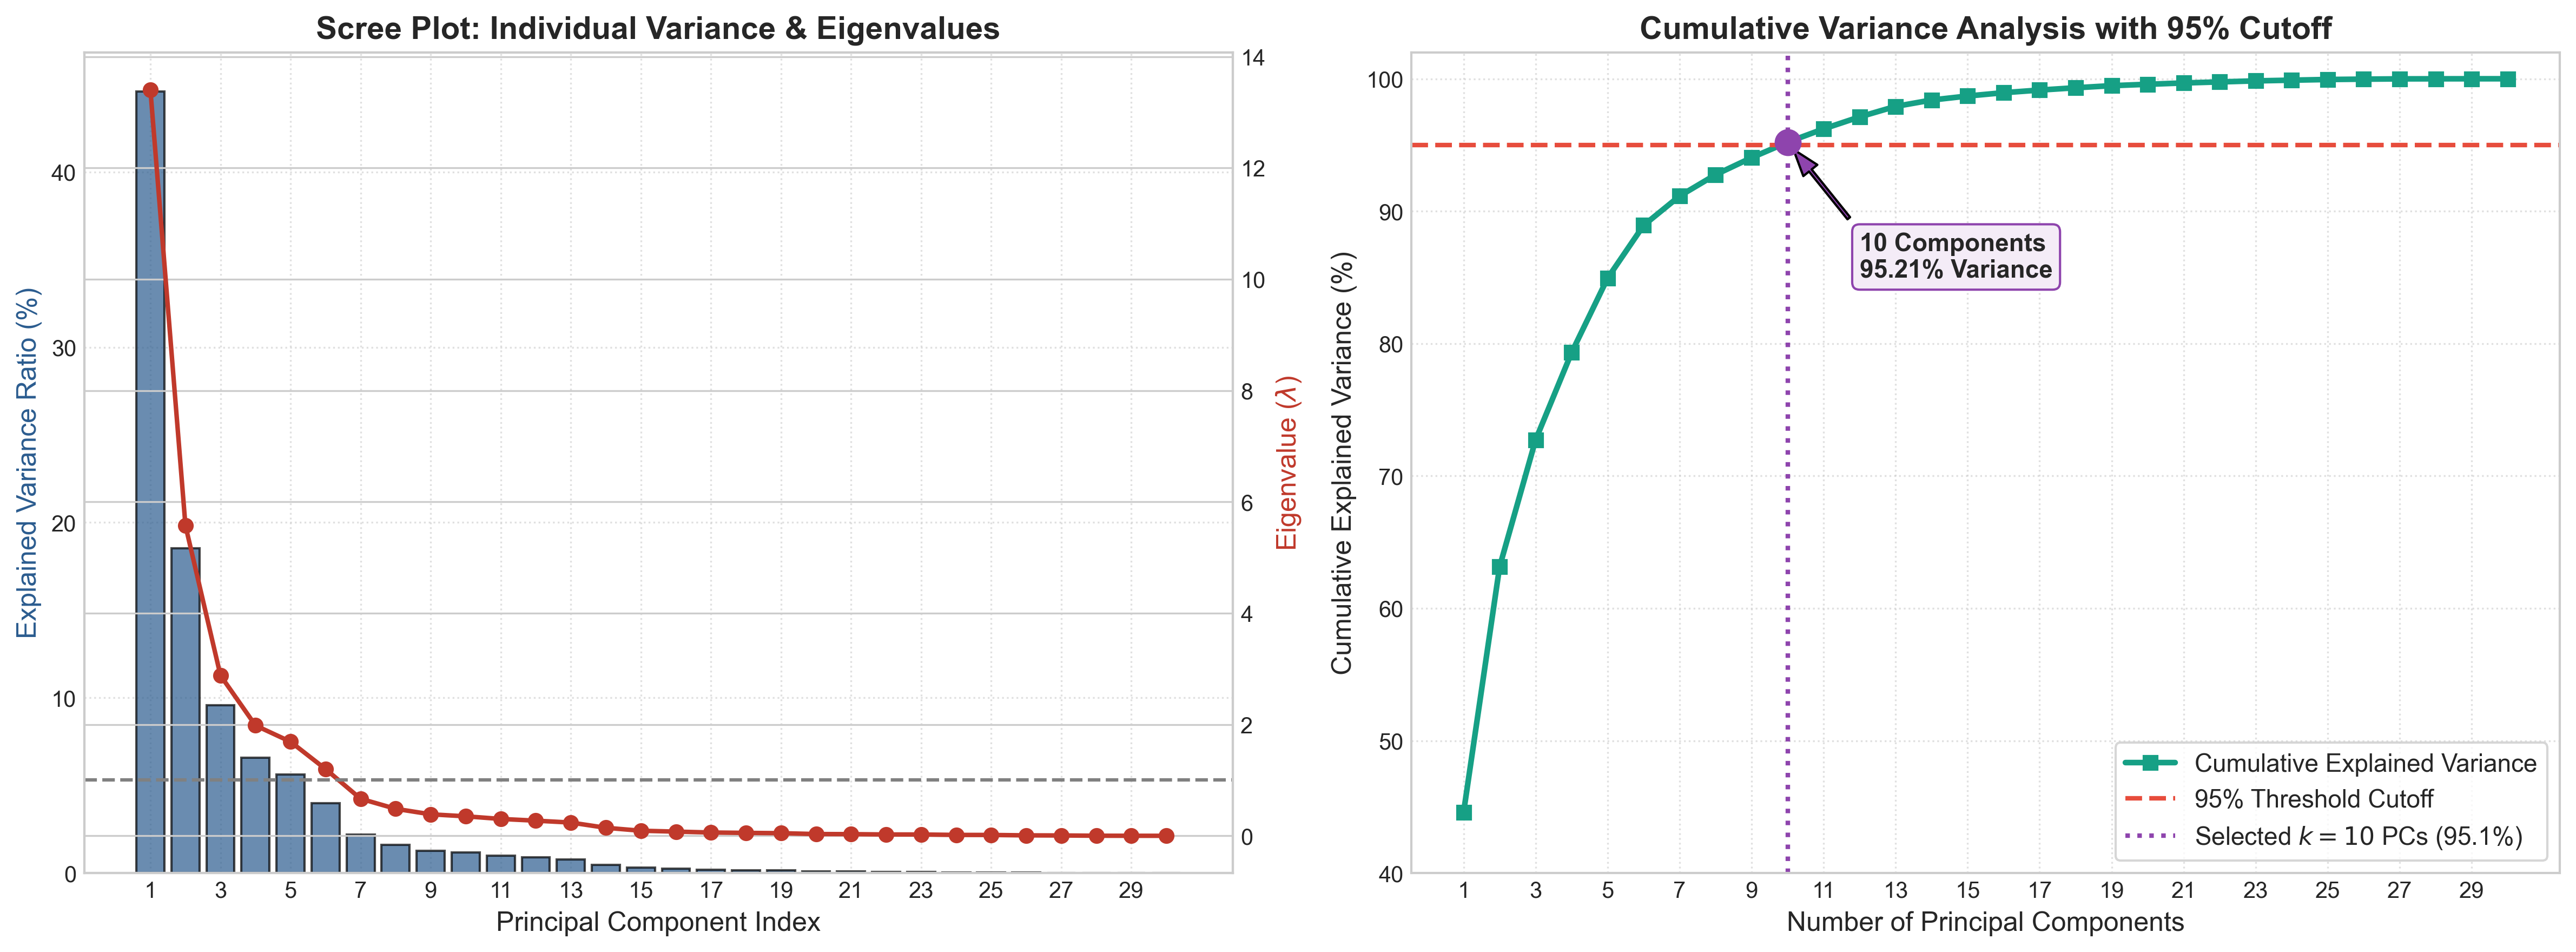
\includegraphics[width=0.98\linewidth]{01_scree_and_cumulative_variance.png}
\caption{Scree Plot (Individual Variance and Eigenvalues) and Cumulative Explained Variance Curve.}
\end{figure}

\begin{figure}[H]
\centering
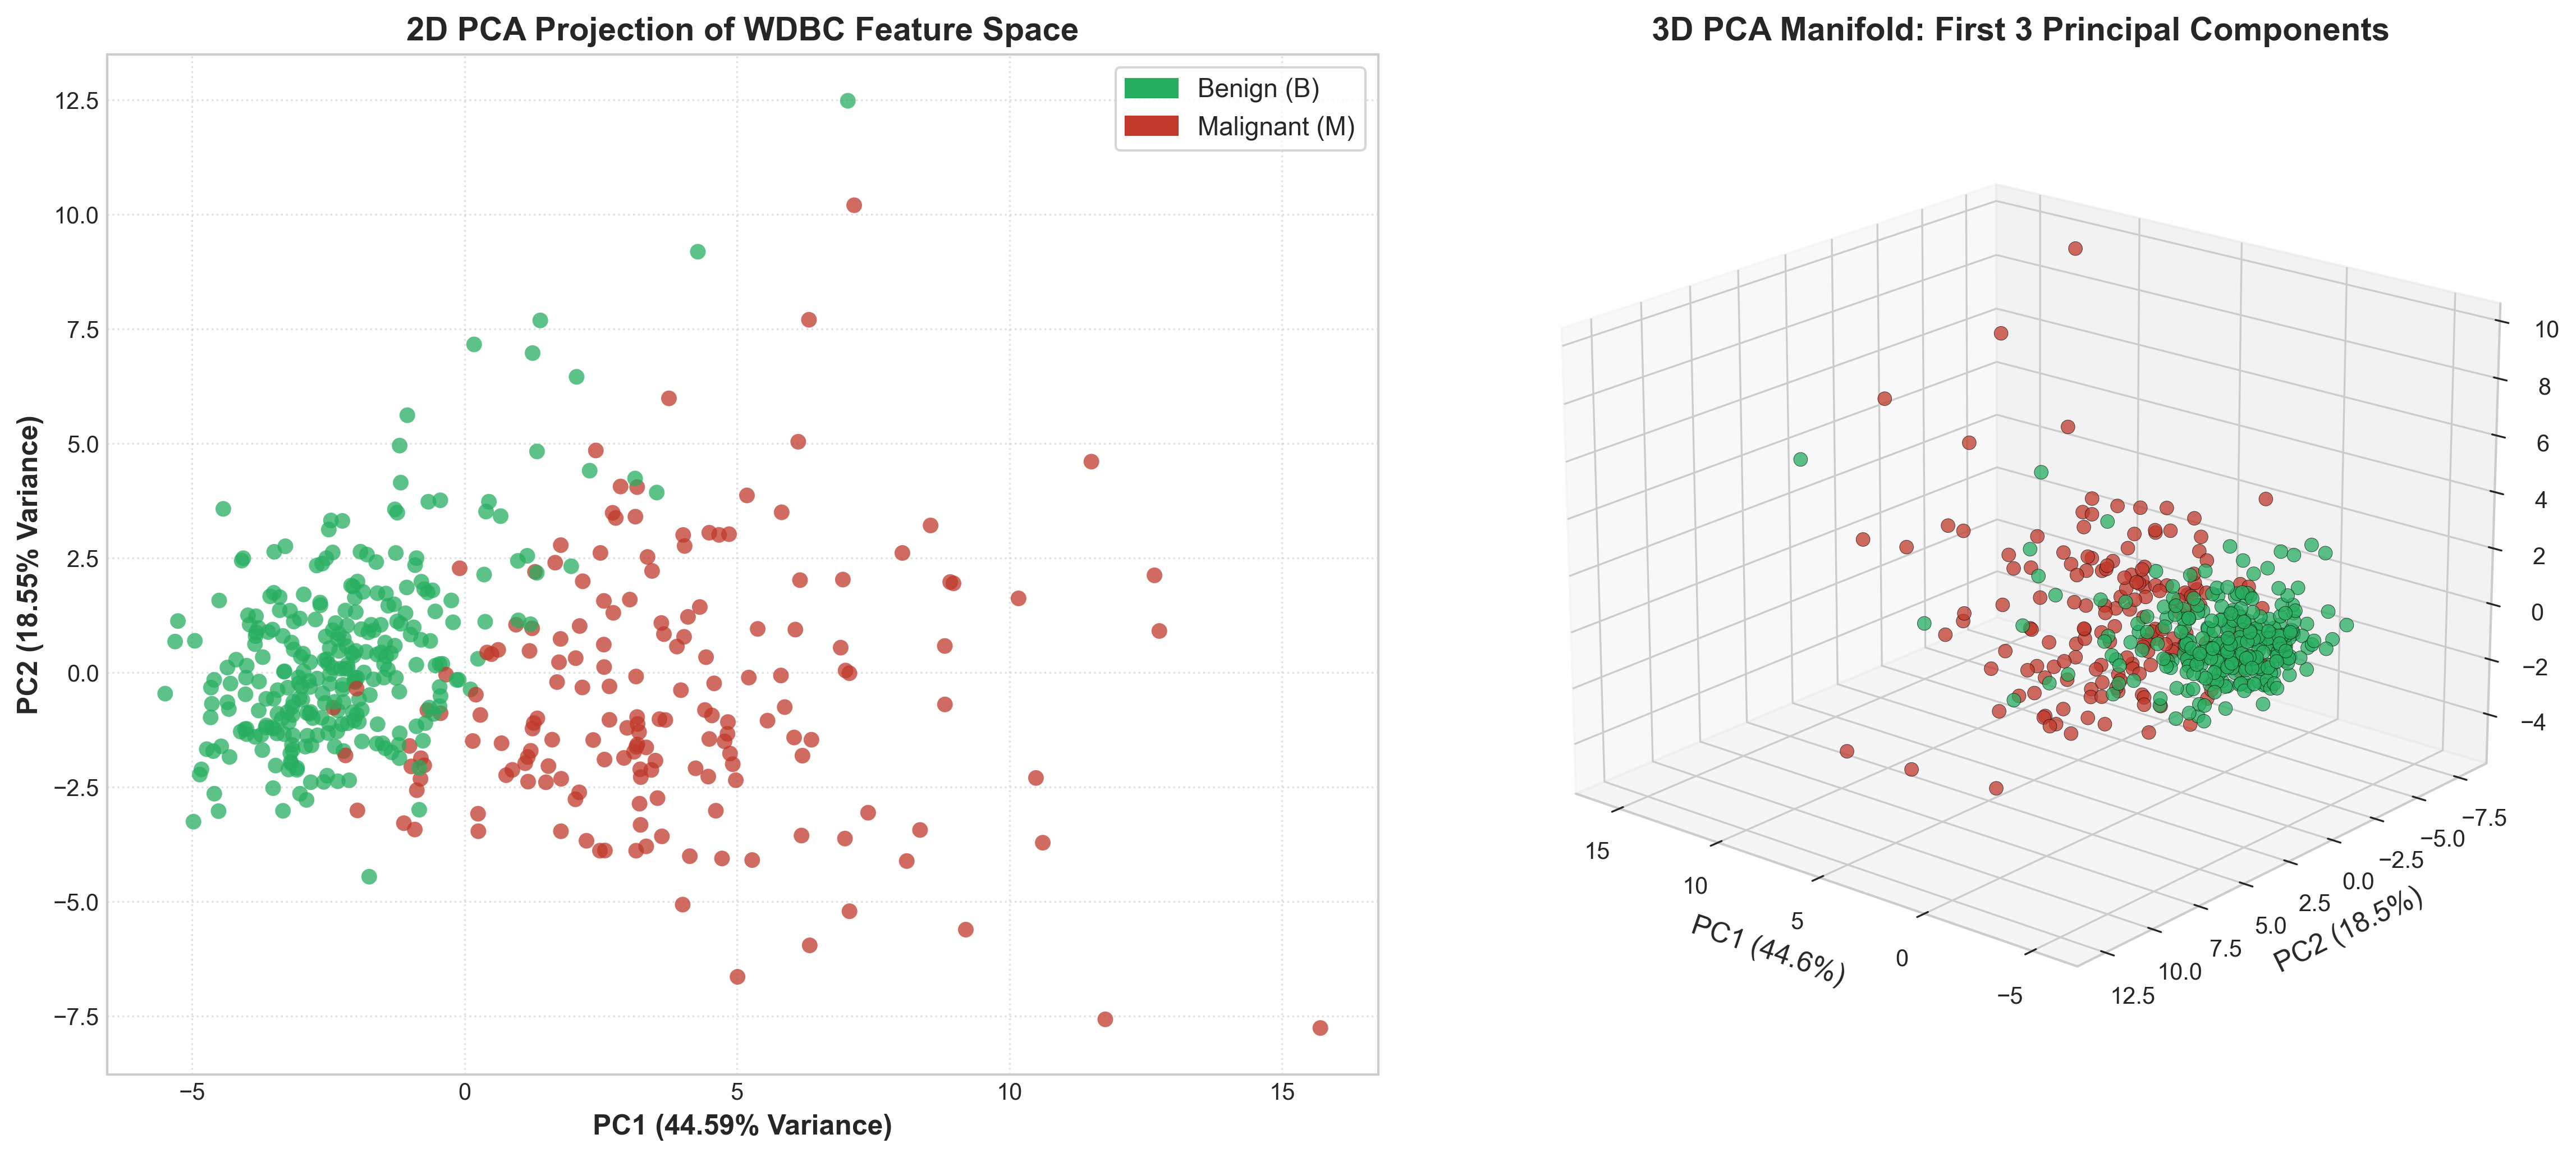
\includegraphics[width=0.98\linewidth]{02_pca_2d_and_3d_projections.png}
\caption{2D and 3D PCA Projections of WDBC Feature Space showing separation between Benign and Malignant tumors.}
\end{figure}

\begin{figure}[H]
\centering
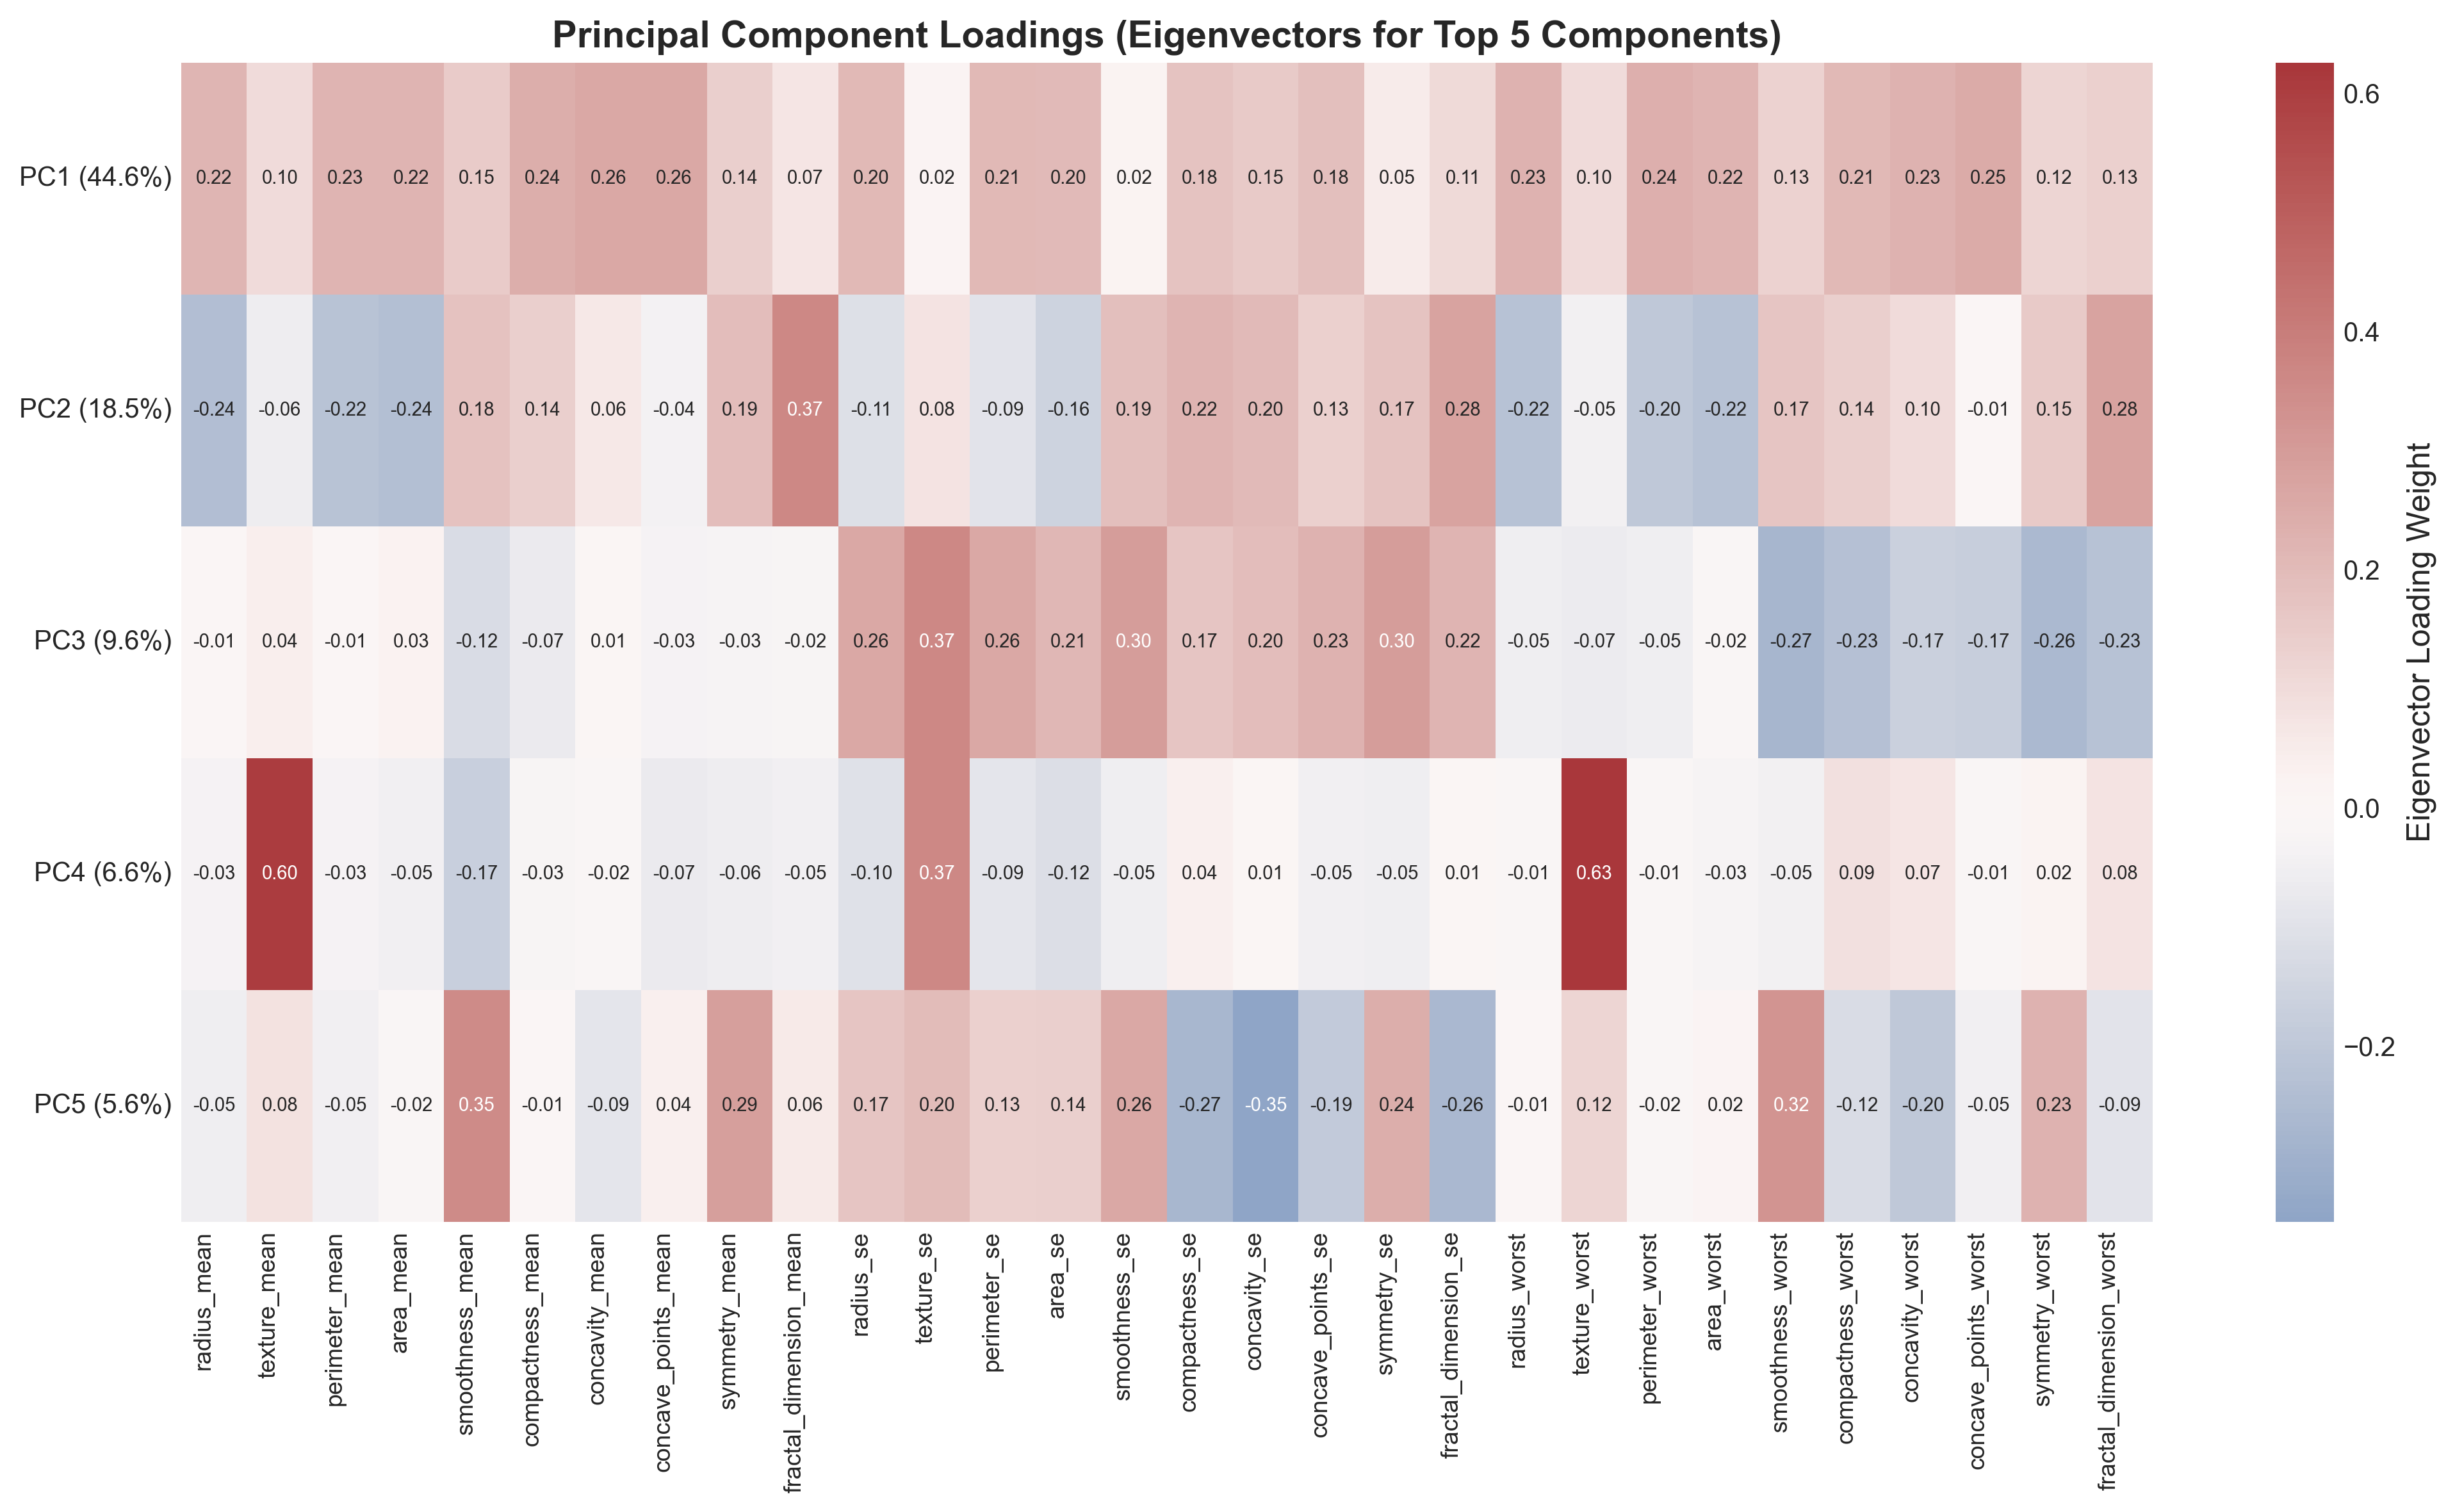
\includegraphics[width=0.98\linewidth]{03_pca_component_loadings_heatmap.png}
\caption{Principal Component Loadings Heatmap for the Top 5 Components across the 30 Continuous Features.}
\end{figure}

\section{Hyperparameter Tuning \& Model Optimization}
Ten machine learning classifiers were tuned and validated under both No-PCA and With-PCA settings using 5-Fold Stratified Cross-Validation.

\subsection{Support Vector Machine (SVM)}
\begin{table}[H]
\centering
\caption{SVM — Hyperparameter Tuning Results}
\begin{tabular}{ccccc}
\toprule
\textbf{Kernel} & \textbf{$C$ Values} & \textbf{$\gamma$ Values} & \textbf{CV Acc (No-PCA)} & \textbf{CV Acc (With-PCA)} \\
\midrule
\textbf{RBF} & \textbf{10} & \textbf{0.01} & \textbf{97.80\%} & \textbf{97.58\%} \\
RBF & 1 & scale & 97.36\% & 97.36\% \\
Linear & 0.1 & N/A & 97.14\% & 96.92\% \\
Linear & 1 & N/A & 96.92\% & 97.14\% \\
Poly & 10 & scale & 94.73\% & 94.95\% \\
\bottomrule
\end{tabular}
\end{table}

\subsection{Gaussian Naïve Bayes}
\begin{table}[H]
\centering
\caption{Gaussian Naïve Bayes — Smoothing Parameter Tuning}
\begin{tabular}{ccc}
\toprule
\textbf{Smoothing Parameter ($\text{var\_smoothing}$)} & \textbf{CV Acc (No-PCA)} & \textbf{CV Acc (With-PCA)} \\
\midrule
\textbf{$10^{-11}$} & \textbf{93.85\%} & \textbf{91.21\%} \\
$10^{-9}$ & 93.85\% & 91.21\% \\
$10^{-7}$ & 93.85\% & 91.21\% \\
$10^{-5}$ & 93.63\% & 91.21\% \\
$10^{-1}$ & 92.53\% & 90.99\% \\
\bottomrule
\end{tabular}
\end{table}

\subsection{k-Nearest Neighbors (KNN)}
\begin{table}[H]
\centering
\caption{KNN — Hyperparameter Tuning Results}
\begin{tabular}{ccccc}
\toprule
\textbf{$k$ Neighbors} & \textbf{Weights} & \textbf{Distance Metric} & \textbf{CV Acc (No-PCA)} & \textbf{CV Acc (With-PCA)} \\
\midrule
\textbf{3} & \textbf{uniform} & \textbf{manhattan} & \textbf{97.58\%} & 96.92\% \\
\textbf{3} & \textbf{uniform} & \textbf{euclidean} & 96.92\% & \textbf{97.14\%} \\
5 & uniform & manhattan & 97.14\% & 96.70\% \\
7 & distance & euclidean & 96.92\% & 96.70\% \\
11 & uniform & euclidean & 96.04\% & 96.48\% \\
21 & uniform & euclidean & 95.60\% & 95.82\% \\
\bottomrule
\end{tabular}
\end{table}

\subsection{Logistic Regression}
\begin{table}[H]
\centering
\caption{Logistic Regression — Hyperparameter Tuning Results}
\begin{tabular}{ccccc}
\toprule
\textbf{Regularization ($C$)} & \textbf{Penalty} & \textbf{Solver} & \textbf{CV Acc (No-PCA)} & \textbf{CV Acc (With-PCA)} \\
\midrule
\textbf{0.10} & \textbf{L2} & \textbf{liblinear} & \textbf{97.36\%} & \textbf{97.80\%} \\
0.10 & L2 & lbfgs & 97.14\% & 97.58\% \\
1.00 & L2 & liblinear & 97.14\% & 97.36\% \\
10.00 & L2 & lbfgs & 96.26\% & 96.70\% \\
\bottomrule
\end{tabular}
\end{table}

\subsection{Decision Tree}
\begin{table}[H]
\centering
\caption{Decision Tree — Hyperparameter Tuning Results}
\begin{tabular}{cccccc}
\toprule
\textbf{Criterion} & \textbf{Max Depth} & \textbf{Min Split} & \textbf{Min Leaf} & \textbf{CV Acc (No-PCA)} & \textbf{CV Acc (With-PCA)} \\
\midrule
\textbf{entropy} & \textbf{5} & \textbf{10} & \textbf{2} & \textbf{93.63\%} & 93.85\% \\
\textbf{entropy} & \textbf{7} & \textbf{5} & \textbf{1} & 92.53\% & \textbf{94.95\%} \\
gini & 5 & 5 & 2 & 92.75\% & 93.19\% \\
gini & None & 2 & 1 & 91.87\% & 92.53\% \\
\bottomrule
\end{tabular}
\end{table}

\subsection{Random Forest, AdaBoost, Gradient Boosting, XGBoost, and Stacking}
\begin{table}[H]
\centering
\caption{Ensemble Models — Optimal Configurations and Tuning Scores}
\resizebox{\linewidth}{!}{
\begin{tabular}{llcc}
\toprule
\textbf{Model} & \textbf{Best Hyperparameters (No-PCA / With-PCA)} & \textbf{CV Acc (No-PCA)} & \textbf{CV Acc (With-PCA)} \\
\midrule
\textbf{Random Forest} & $T=100, d=5$ (No-PCA) / $T=50, d=\text{None}$ (PCA) & 96.70\% & 96.04\% \\
\textbf{AdaBoost} & $M=100, \eta=0.50$ (SAMME) & 97.14\% & 97.14\% \\
\textbf{Gradient Boosting} & $M=200, \eta=0.10, d=2$ (No-PCA) / $\eta=0.20$ (PCA) & 97.36\% & 96.26\% \\
\textbf{XGBoost} & $M=200, \eta=0.10, d=3$ (No-PCA) / $M=100, \eta=0.20$ (PCA) & 97.36\% & \textbf{97.80\%} \\
\textbf{Stacking} & Base: [SVM, NB, KNN, RF] $\to$ Meta: Logistic Regression & \textbf{98.02\%} & \textbf{98.02\%} \\
\bottomrule
\end{tabular}
}
\end{table}

\begin{figure}[H]
\centering
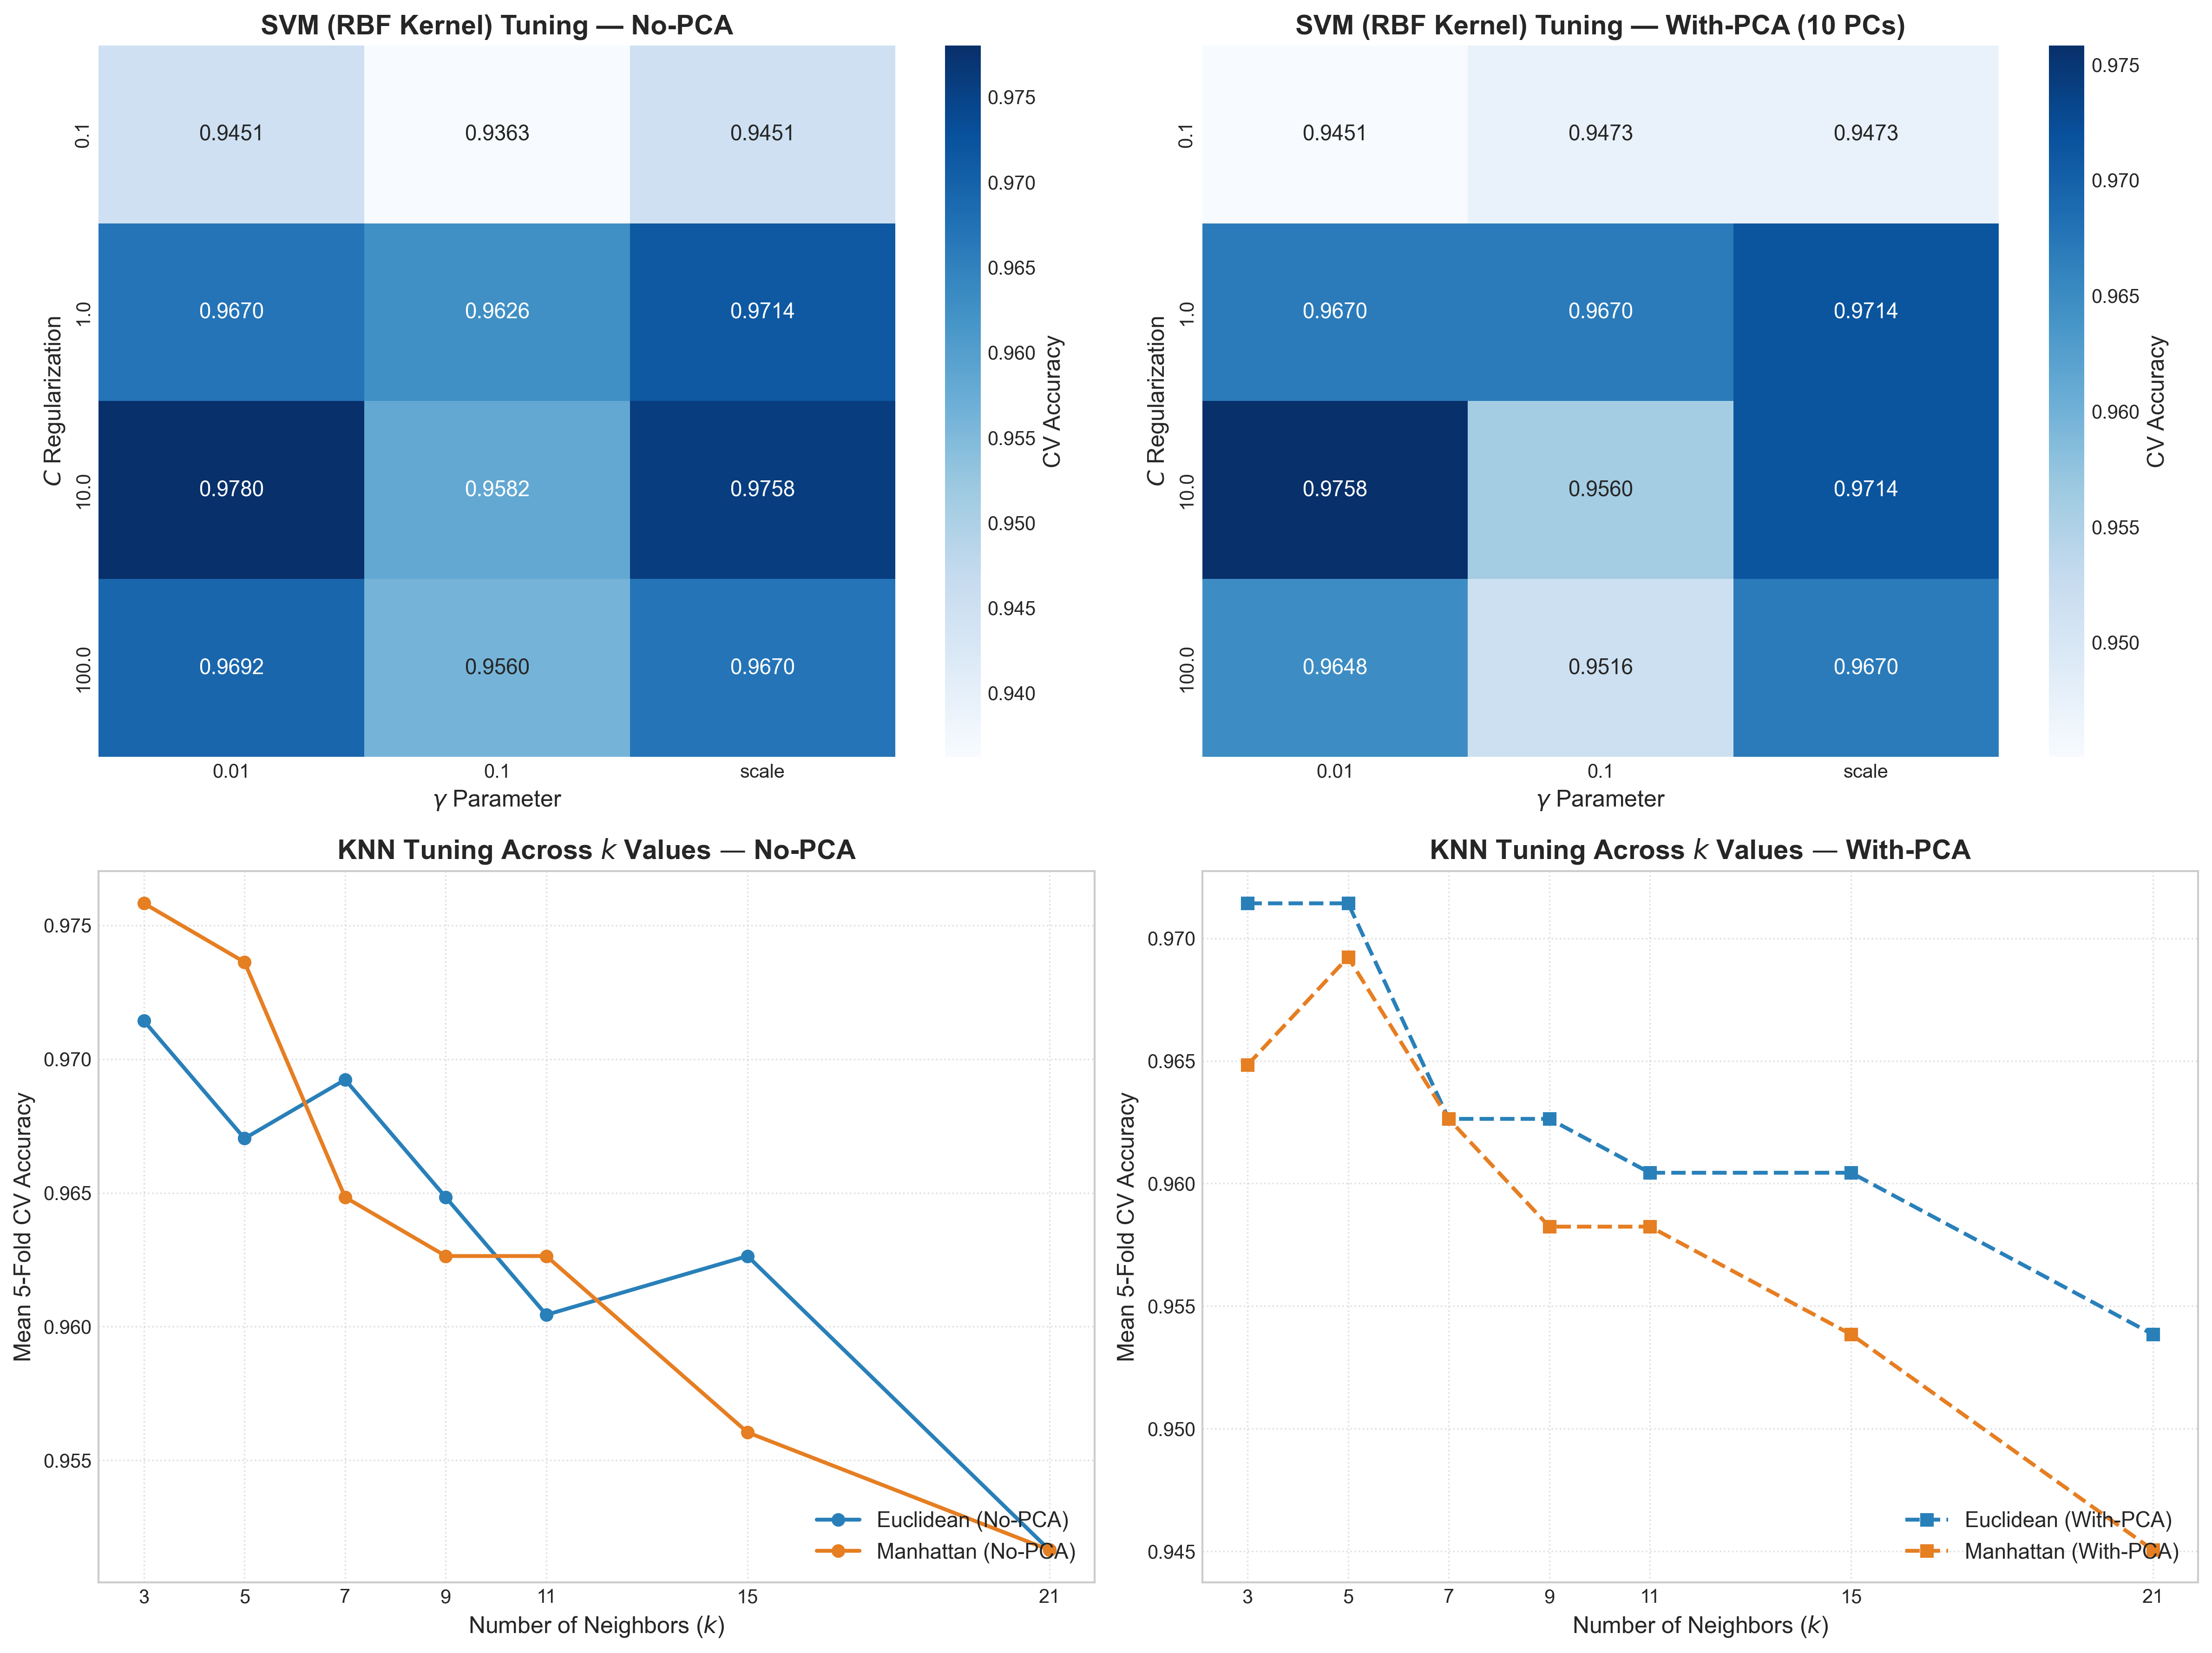
\includegraphics[width=0.98\linewidth]{04_svm_knn_tuning_heatmaps.png}
\caption{Hyperparameter Response Surfaces for SVM ($C$ vs $\gamma$) and KNN ($k$ vs metric) under No-PCA vs With-PCA.}
\end{figure}

\begin{figure}[H]
\centering
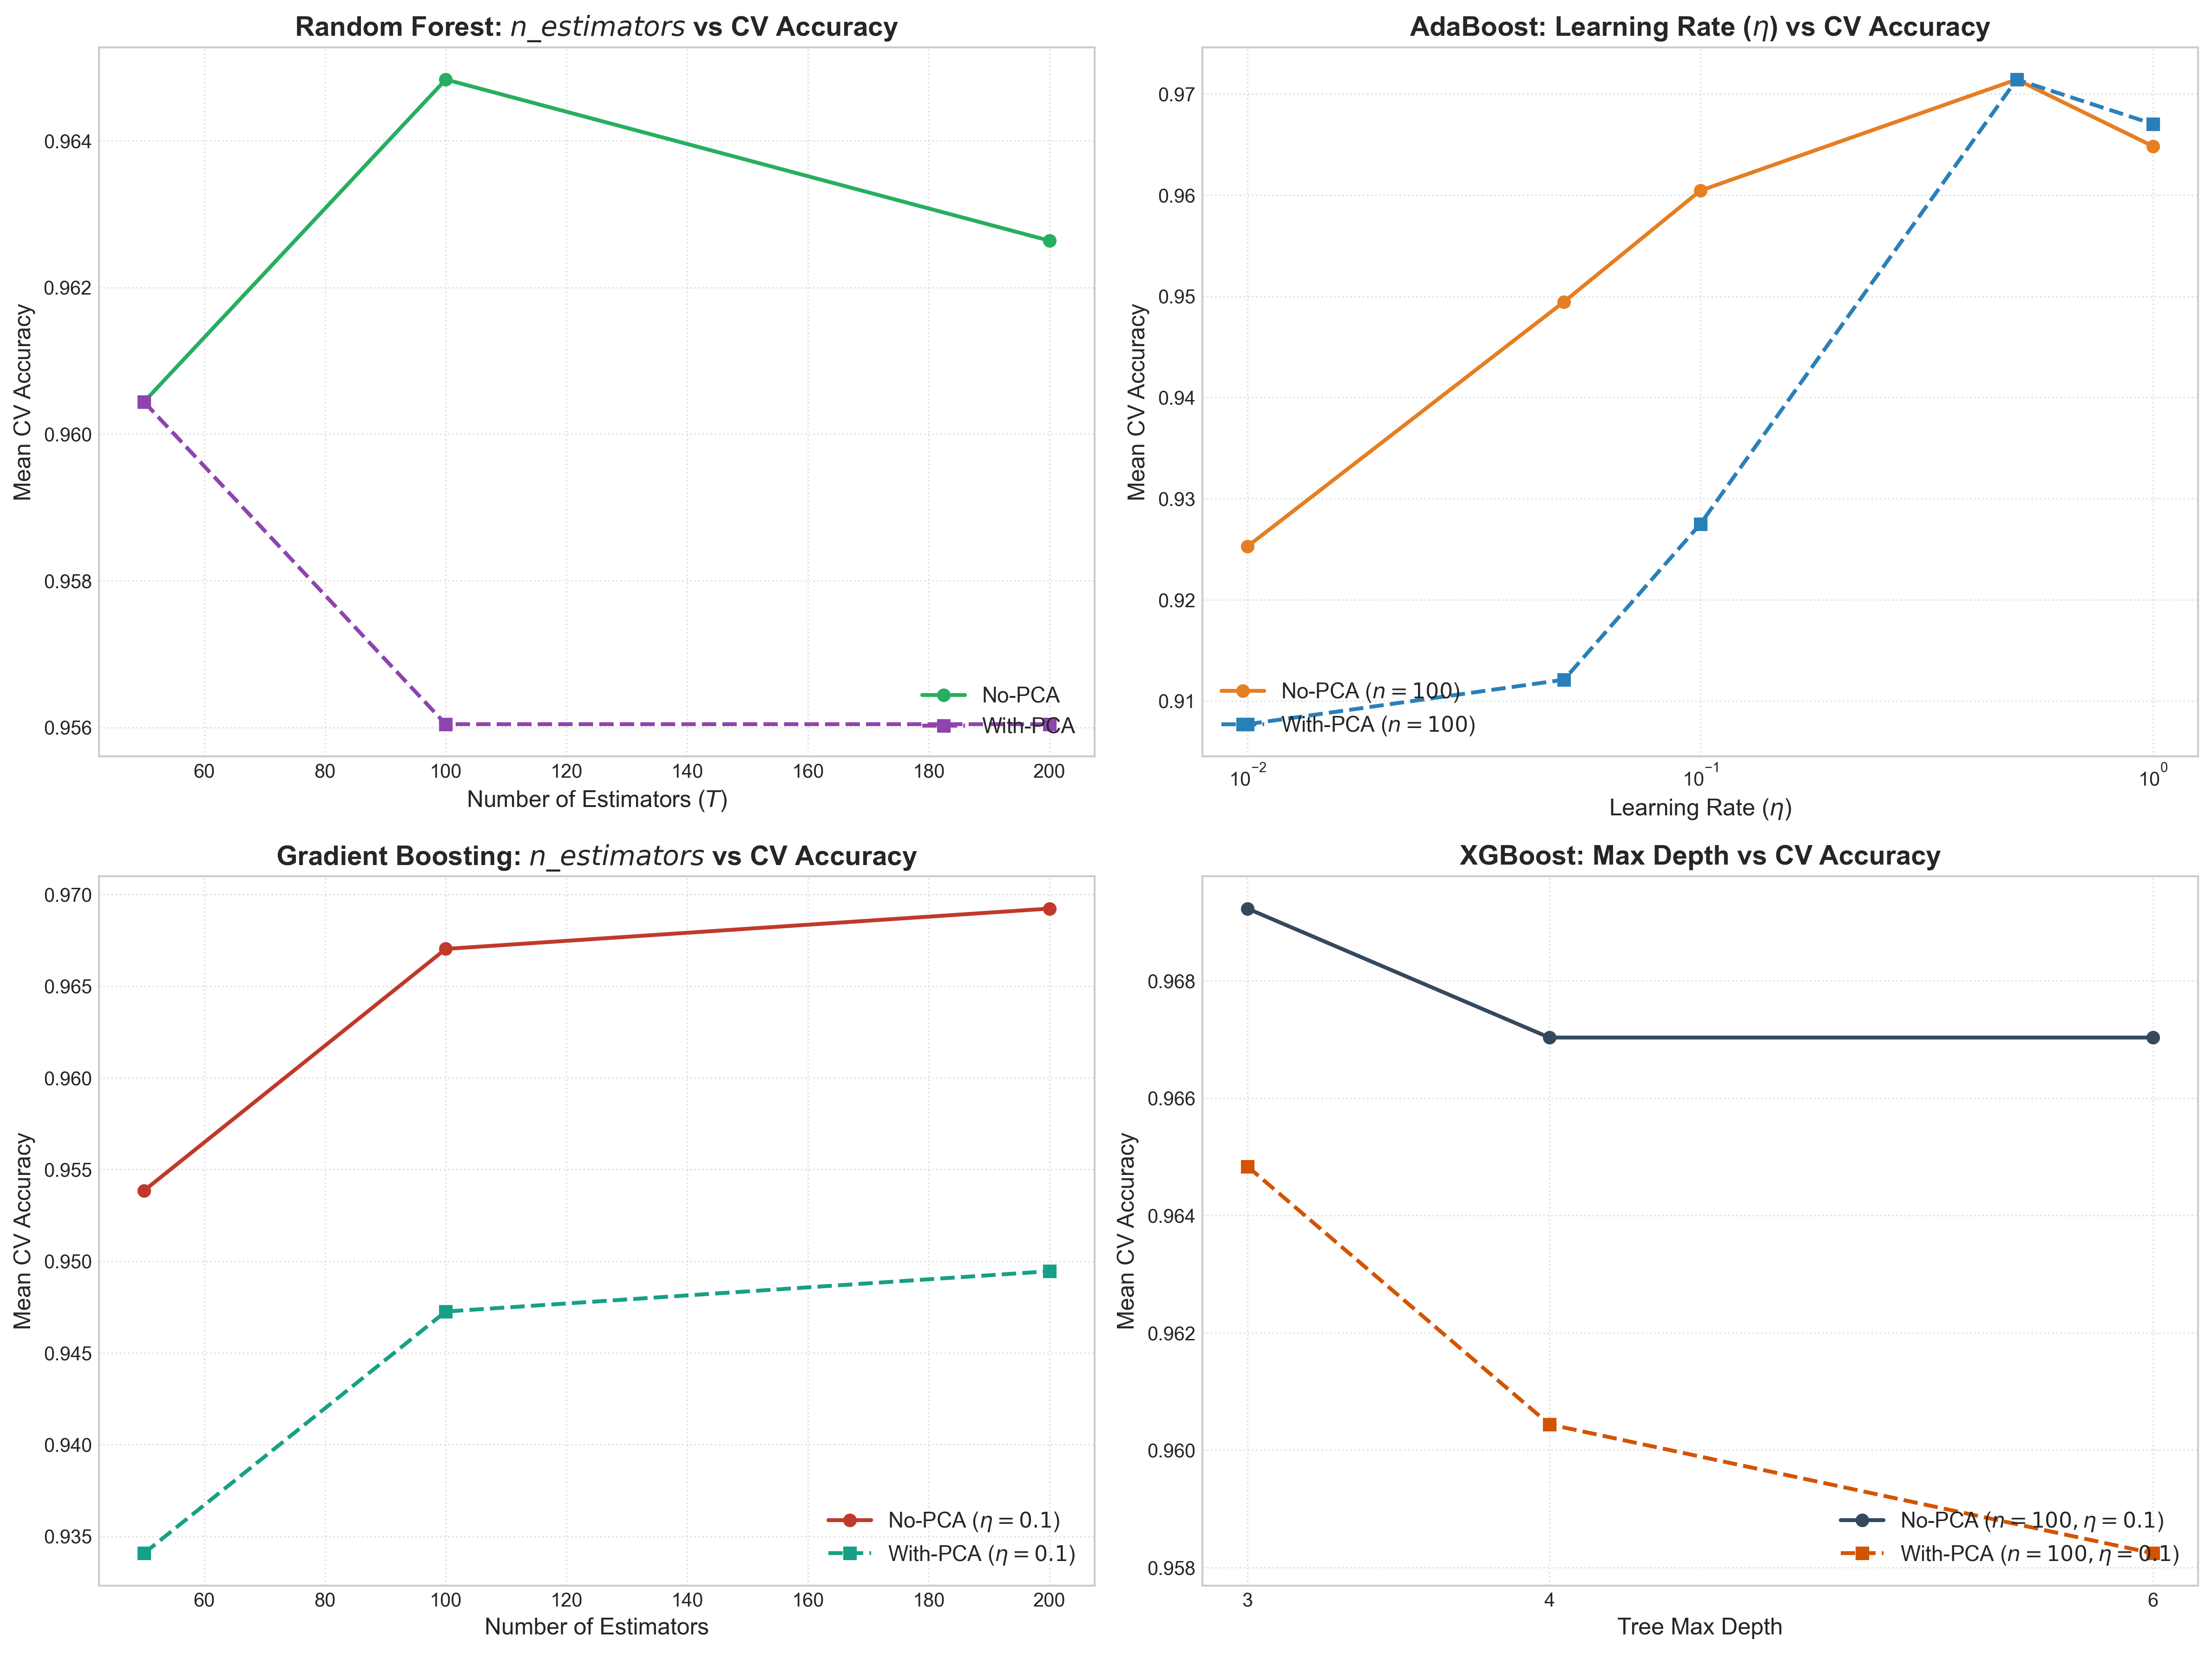
\includegraphics[width=0.98\linewidth]{05_tree_ensemble_tuning_comparison.png}
\caption{Hyperparameter Tuning Curves for Tree Ensembles (Random Forest, AdaBoost, Gradient Boosting, XGBoost).}
\end{figure}

\section{5-Fold Stratified Cross-Validation Results}
Table~\ref{tab:cv_results} records the fold-by-fold accuracy, average score, and cross-fold standard deviation across all 10 evaluated models.

\begin{table}[H]
\centering
\caption{5-Fold Stratified Cross-Validation Results (No-PCA vs With-PCA)}
\label{tab:cv_results}
\resizebox{\textwidth}{!}{
\begin{tabular}{lcccccccc}
\toprule
\textbf{Model} & \textbf{Fold 1} & \textbf{Fold 2} & \textbf{Fold 3} & \textbf{Fold 4} & \textbf{Fold 5} & \textbf{Avg (No-PCA)} & \textbf{Avg (With-PCA)} & \textbf{Stability ($\Delta \sigma$)} \\
\midrule
\textbf{SVM (RBF)} & 95.6\% & 97.8\% & 98.9\% & 97.8\% & 98.9\% & 97.80\% $\pm 1.20\%$ & 97.58\% $\pm \mathbf{0.82\%}$ & $+0.38\%$ (More Stable) \\
\textbf{Naïve Bayes} & 95.6\% & 97.8\% & 91.2\% & 91.2\% & 93.4\% & 93.85\% $\pm 2.56\%$ & 91.21\% $\pm 3.03\%$ & $-0.47\%$ \\
\textbf{KNN} & 96.7\% & 100.0\% & 96.7\% & 95.6\% & 98.9\% & 97.58\% $\pm 1.62\%$ & 97.14\% $\pm \mathbf{1.49\%}$ & $+0.12\%$ (More Stable) \\
\textbf{Logistic Regression} & 95.6\% & 96.7\% & 97.8\% & 97.8\% & 98.9\% & 97.36\% $\pm 1.12\%$ & \textbf{97.80\% $\pm \mathbf{0.70\%}$} & $+0.43\%$ (More Stable) \\
\textbf{Decision Tree} & 90.1\% & 95.6\% & 91.2\% & 95.6\% & 95.6\% & 93.63\% $\pm 2.45\%$ & \textbf{94.95\% $\pm \mathbf{1.64\%}$} & $+0.80\%$ (More Stable) \\
\textbf{Random Forest} & 96.7\% & 100.0\% & 94.5\% & 94.5\% & 97.8\% & 96.70\% $\pm 2.09\%$ & 96.04\% $\pm \mathbf{1.64\%}$ & $+0.44\%$ (More Stable) \\
\textbf{AdaBoost} & 95.6\% & 96.7\% & 96.7\% & 97.8\% & 98.9\% & 97.14\% $\pm 1.12\%$ & 97.14\% $\pm \mathbf{0.54\%}$ & $+0.58\%$ (More Stable) \\
\textbf{Gradient Boosting} & 96.7\% & 97.8\% & 96.7\% & 96.7\% & 98.9\% & 97.36\% $\pm 0.88\%$ & 96.26\% $\pm 1.49\%$ & $-0.61\%$ \\
\textbf{XGBoost} & 97.8\% & 96.7\% & 96.7\% & 96.7\% & 98.9\% & 97.36\% $\pm 0.88\%$ & \textbf{97.80\%} $\pm 1.20\%$ & $-0.32\%$ \\
\textbf{Stacking} & 96.7\% & 98.9\% & 97.8\% & 97.8\% & 98.9\% & \textbf{98.02\% $\pm 0.82\%$} & \textbf{98.02\%} $\pm 1.08\%$ & $-0.25\%$ \\
\bottomrule
\end{tabular}
}
\end{table}

\begin{figure}[H]
\centering
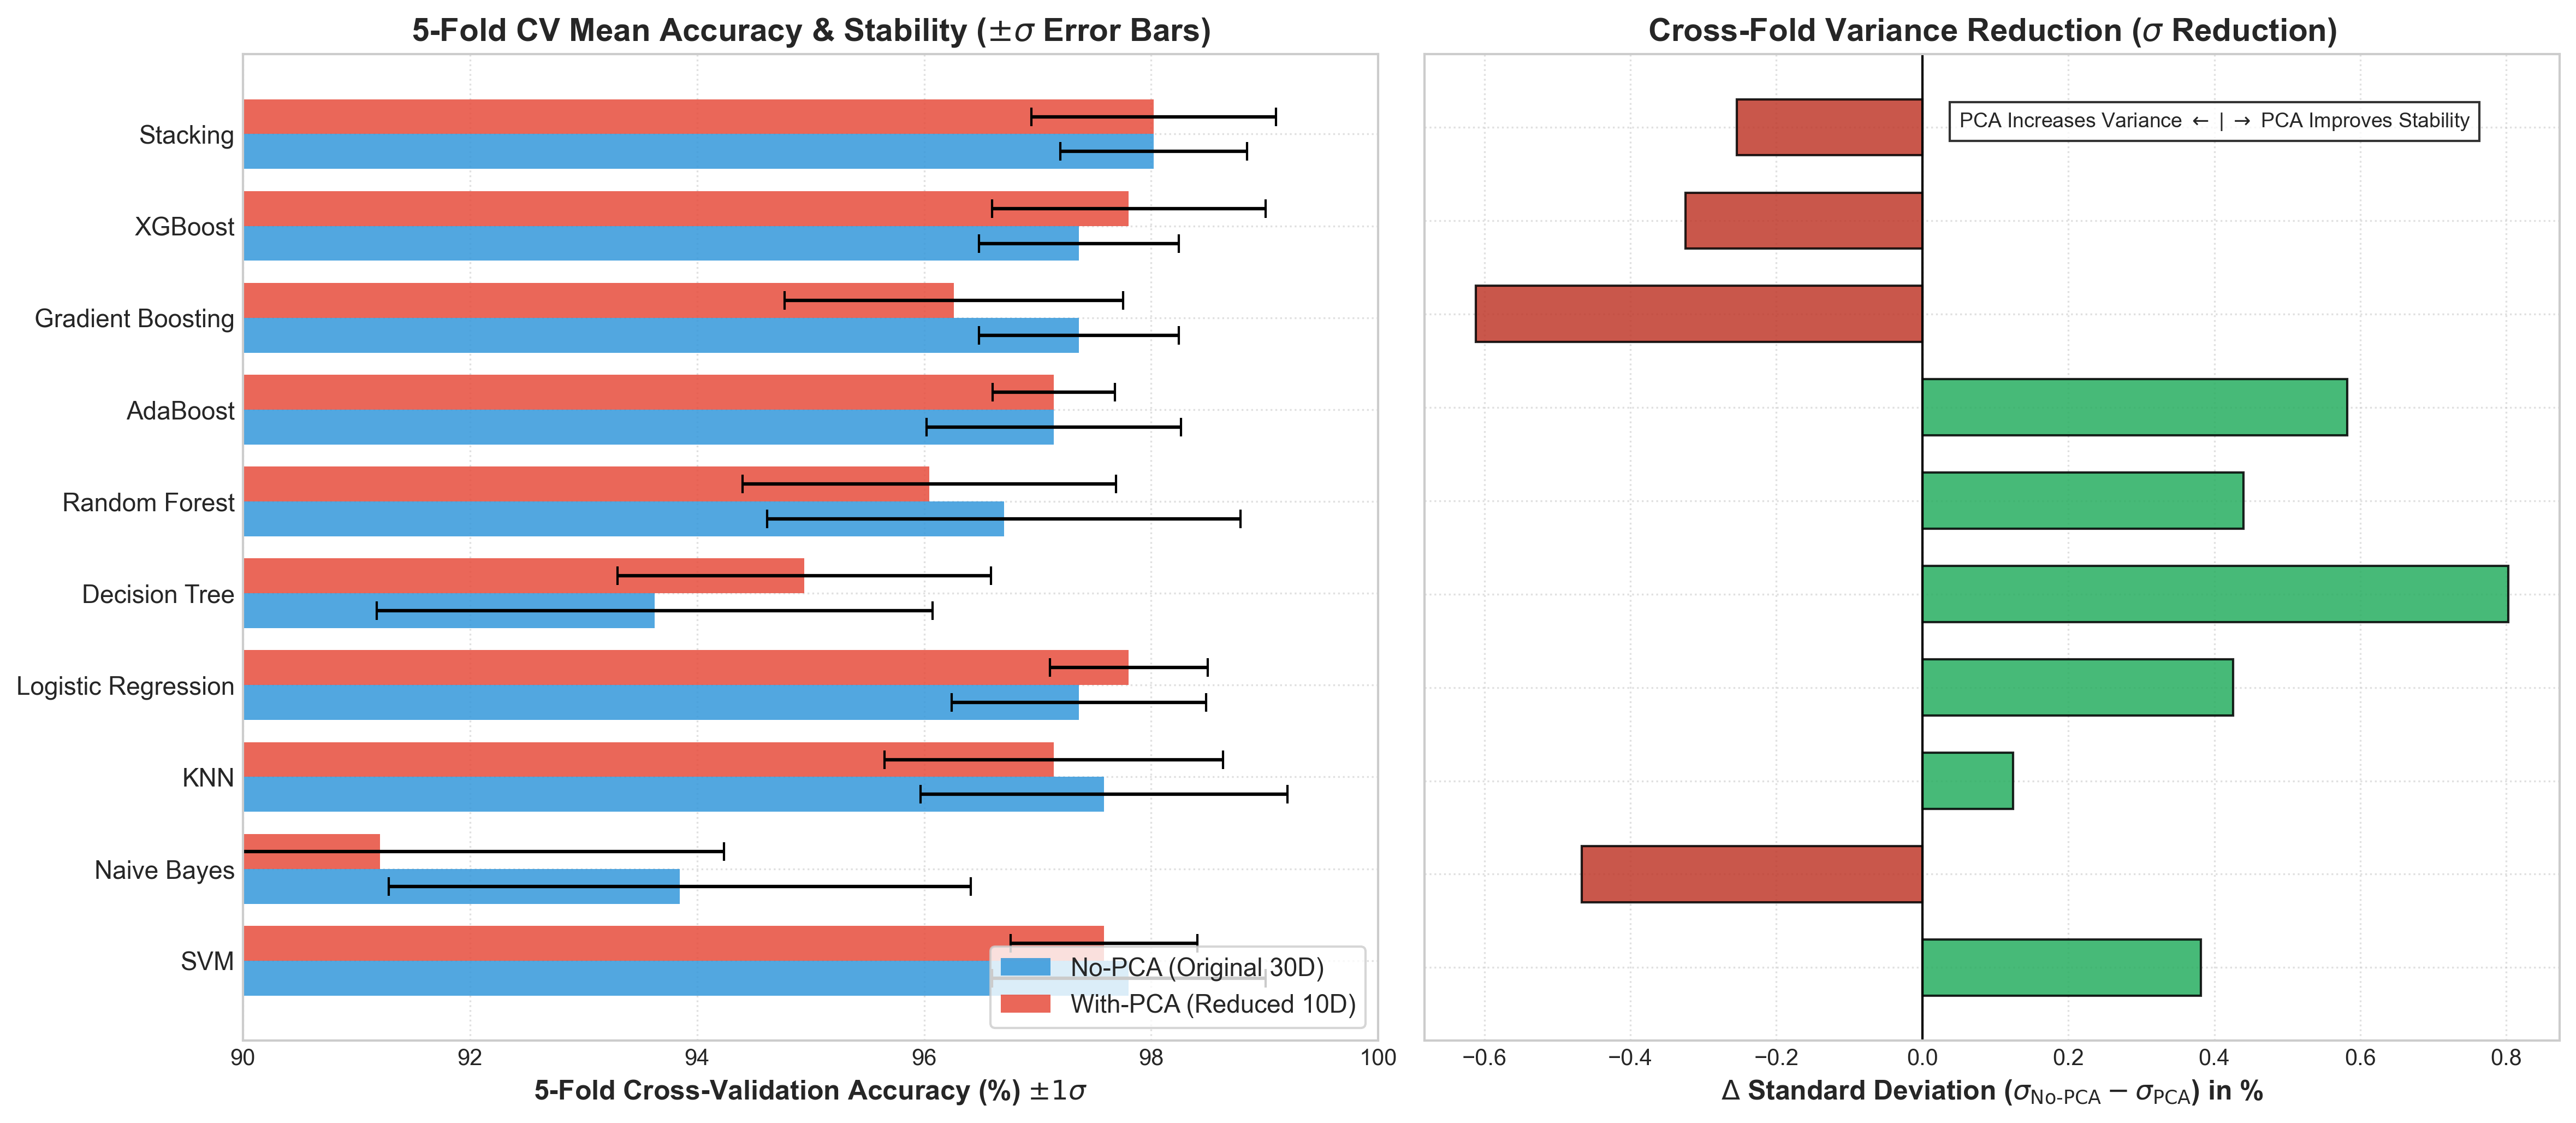
\includegraphics[width=0.98\linewidth]{06_5fold_cv_foldwise_comparison.png}
\caption{5-Fold Cross-Validation Accuracy Comparison and Cross-Fold Variance Reduction ($\sigma$ Reduction).}
\end{figure}

\section{Held-out Test Set Benchmarking}
Table~\ref{tab:test_benchmark} summarizes the classification metrics evaluated on the 20\% independent test set ($N=114$ samples).

\begin{table}[H]
\centering
\caption{Held-out Test Set Evaluation ($N=114$ Samples, Benign=72, Malignant=42)}
\label{tab:test_benchmark}
\resizebox{\textwidth}{!}{
\begin{tabular}{lcccccccc}
\toprule
\textbf{Model} & \textbf{Setting} & \textbf{Test Accuracy} & \textbf{Precision} & \textbf{Recall} & \textbf{F1-Score} & \textbf{ROC-AUC} & \textbf{Specificity} & \textbf{Log Loss} \\
\midrule
\textbf{SVM (RBF)} & No-PCA & \textbf{98.25\%} & 100.0\% & 95.24\% & \textbf{97.56\%} & 0.9960 & 100.0\% & 0.0708 \\
& With-PCA & 97.37\% & 100.0\% & 92.86\% & 96.30\% & \textbf{0.9980} & 100.0\% & 0.0716 \\
\textbf{Naïve Bayes} & No-PCA & 92.11\% & 92.31\% & 85.71\% & 88.89\% & 0.9891 & 95.83\% & 0.4999 \\
& With-PCA & 89.47\% & 85.71\% & 85.71\% & 85.71\% & 0.9613 & 91.67\% & 0.3074 \\
\textbf{KNN} & No-PCA & 96.49\% & 100.0\% & 90.48\% & 95.00\% & 0.9735 & 100.0\% & 0.6501 \\
& With-PCA & 94.74\% & 97.37\% & 88.10\% & 92.50\% & 0.9780 & 98.61\% & 0.6694 \\
\textbf{Logistic Regression} & No-PCA & \textbf{98.25\%} & 100.0\% & 95.24\% & \textbf{97.56\%} & 0.9977 & 100.0\% & 0.0923 \\
& \textbf{With-PCA} & \textbf{98.25\%} & 100.0\% & 95.24\% & \textbf{97.56\%} & \textbf{0.9980} & 100.0\% & 0.0940 \\
\textbf{Decision Tree} & No-PCA & 96.49\% & 100.0\% & 90.48\% & 95.00\% & 0.9744 & 100.0\% & 0.6559 \\
& With-PCA & 94.74\% & 97.37\% & 88.10\% & 92.50\% & 0.9560 & 98.61\% & 1.2312 \\
\textbf{Random Forest} & No-PCA & 97.37\% & 100.0\% & 92.86\% & 96.30\% & 0.9950 & 100.0\% & 0.1127 \\
& With-PCA & 94.74\% & 95.00\% & 90.48\% & 92.68\% & 0.9944 & 97.22\% & 0.1433 \\
\textbf{AdaBoost} & No-PCA & 97.37\% & 100.0\% & 92.86\% & 96.30\% & 0.9858 & 100.0\% & 0.3932 \\
& With-PCA & 94.74\% & 97.37\% & 88.10\% & 92.50\% & 0.9934 & 98.61\% & 0.4225 \\
\textbf{Gradient Boosting} & No-PCA & 96.49\% & 100.0\% & 90.48\% & 95.00\% & 0.9934 & 100.0\% & 0.1129 \\
& With-PCA & 95.61\% & 97.44\% & 90.48\% & 93.83\% & 0.9901 & 98.61\% & 0.1414 \\
\textbf{XGBoost} & No-PCA & 97.37\% & 100.0\% & 92.86\% & 96.30\% & 0.9921 & 100.0\% & 0.0982 \\
& \textbf{With-PCA} & \textbf{97.37\%} & 97.56\% & \textbf{95.24\%} & \textbf{96.39\%} & \textbf{0.9921} & 98.61\% & \textbf{0.0934} \\
\textbf{Stacking} & No-PCA & \textbf{98.25\%} & 100.0\% & 95.24\% & \textbf{97.56\%} & 0.9960 & 100.0\% & 0.0784 \\
& With-PCA & 95.61\% & 97.44\% & 90.48\% & 93.83\% & 0.9944 & 98.61\% & 0.0941 \\
\bottomrule
\end{tabular}
}
\end{table}

\begin{figure}[H]
\centering
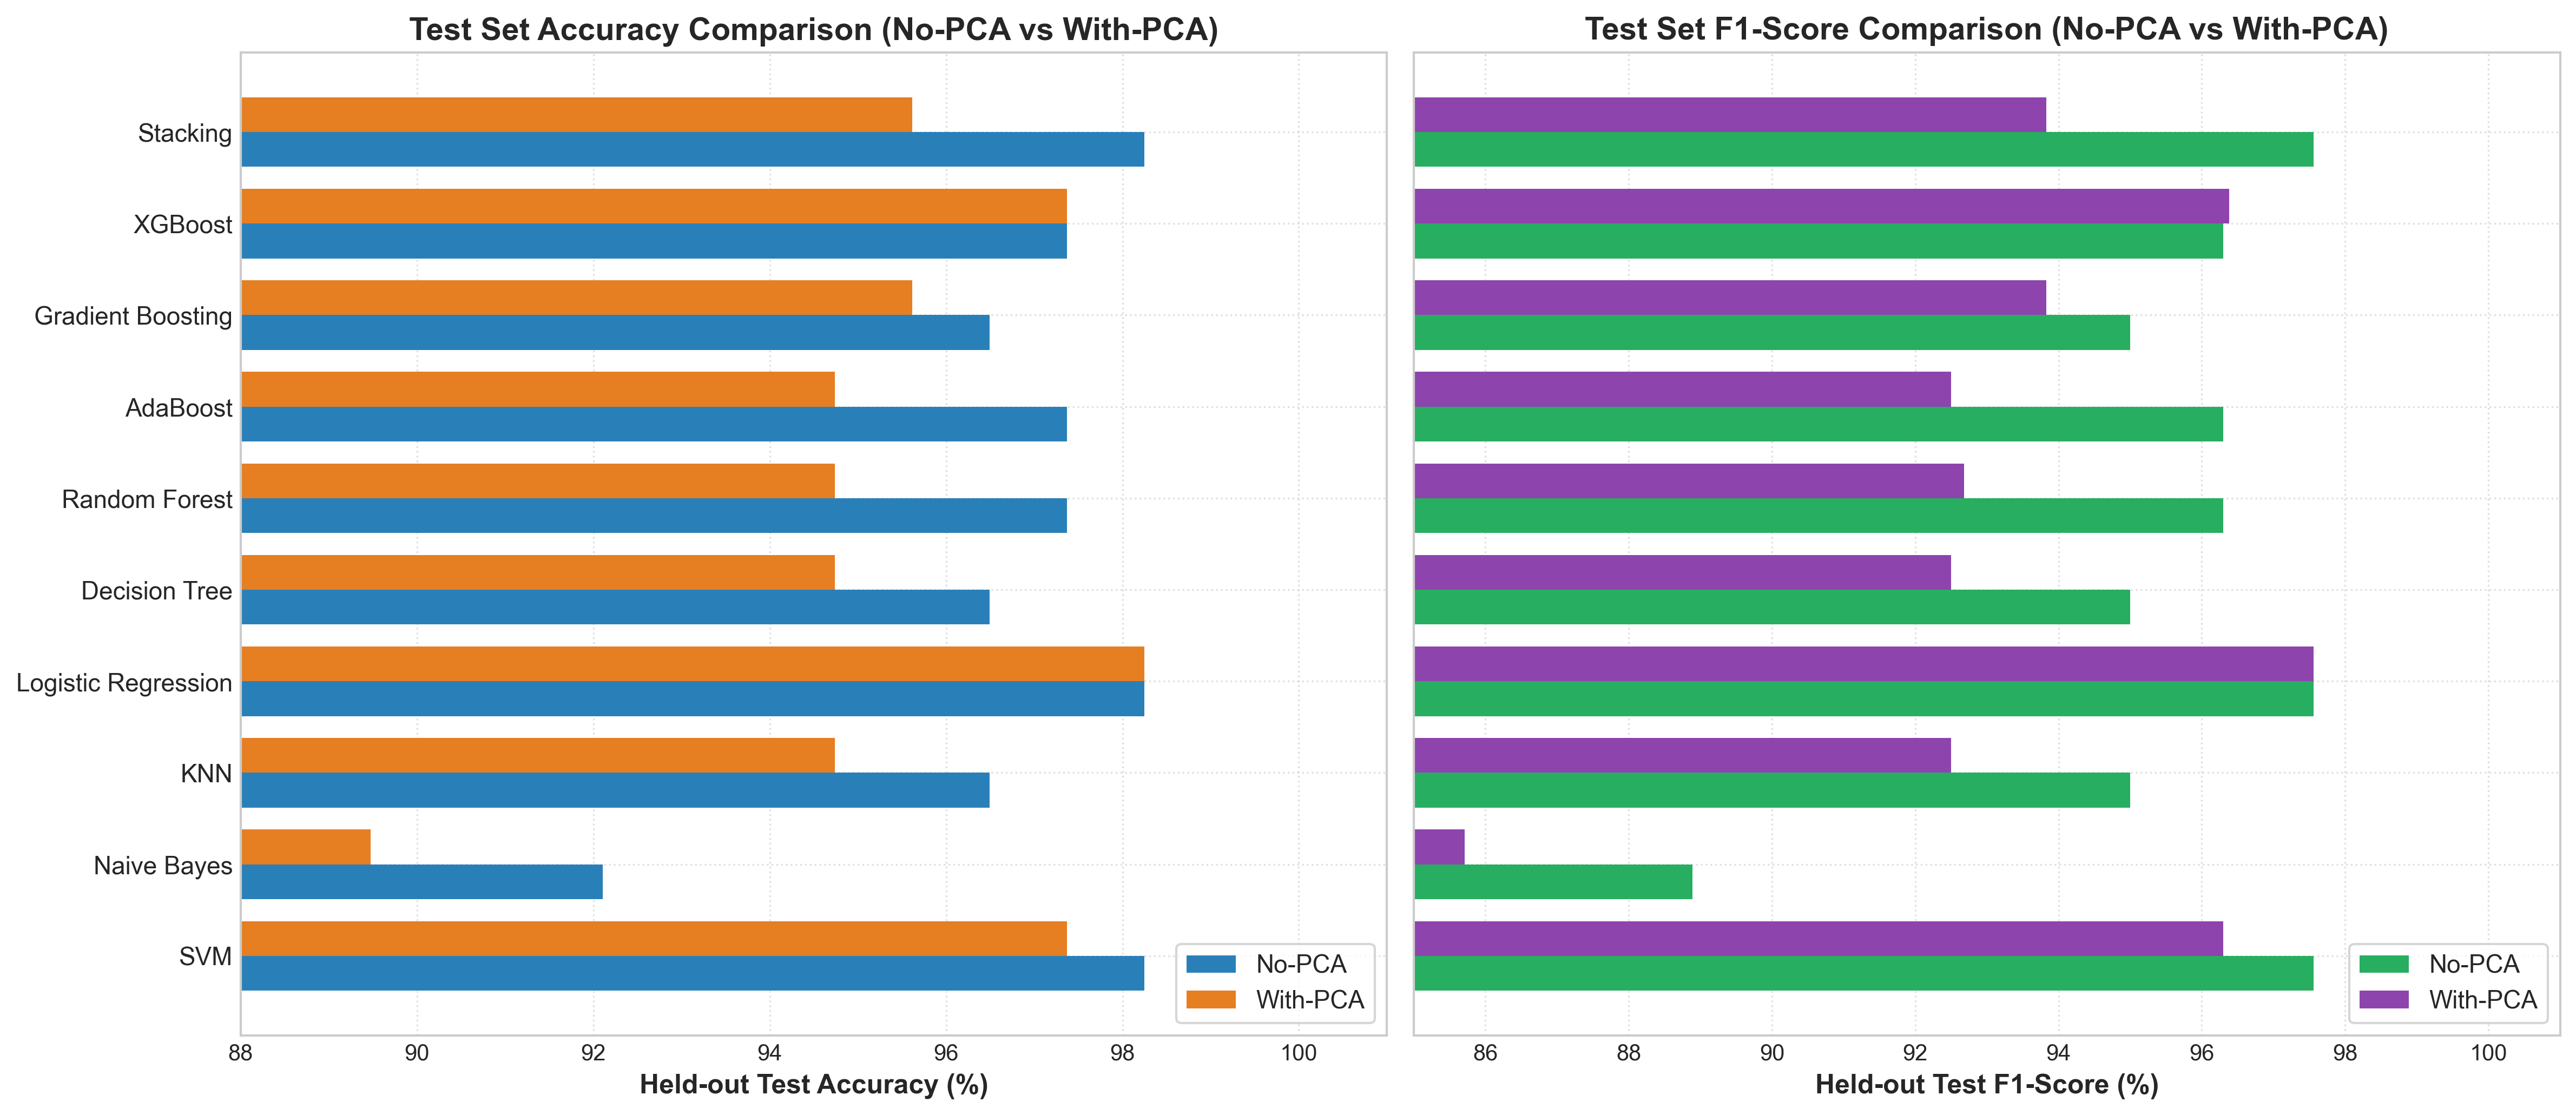
\includegraphics[width=0.98\linewidth]{07_model_performance_comparison_bars.png}
\caption{Held-out Test Set Accuracy and F1-Score Comparison across All 10 Classifiers.}
\end{figure}

\begin{figure}[H]
\centering
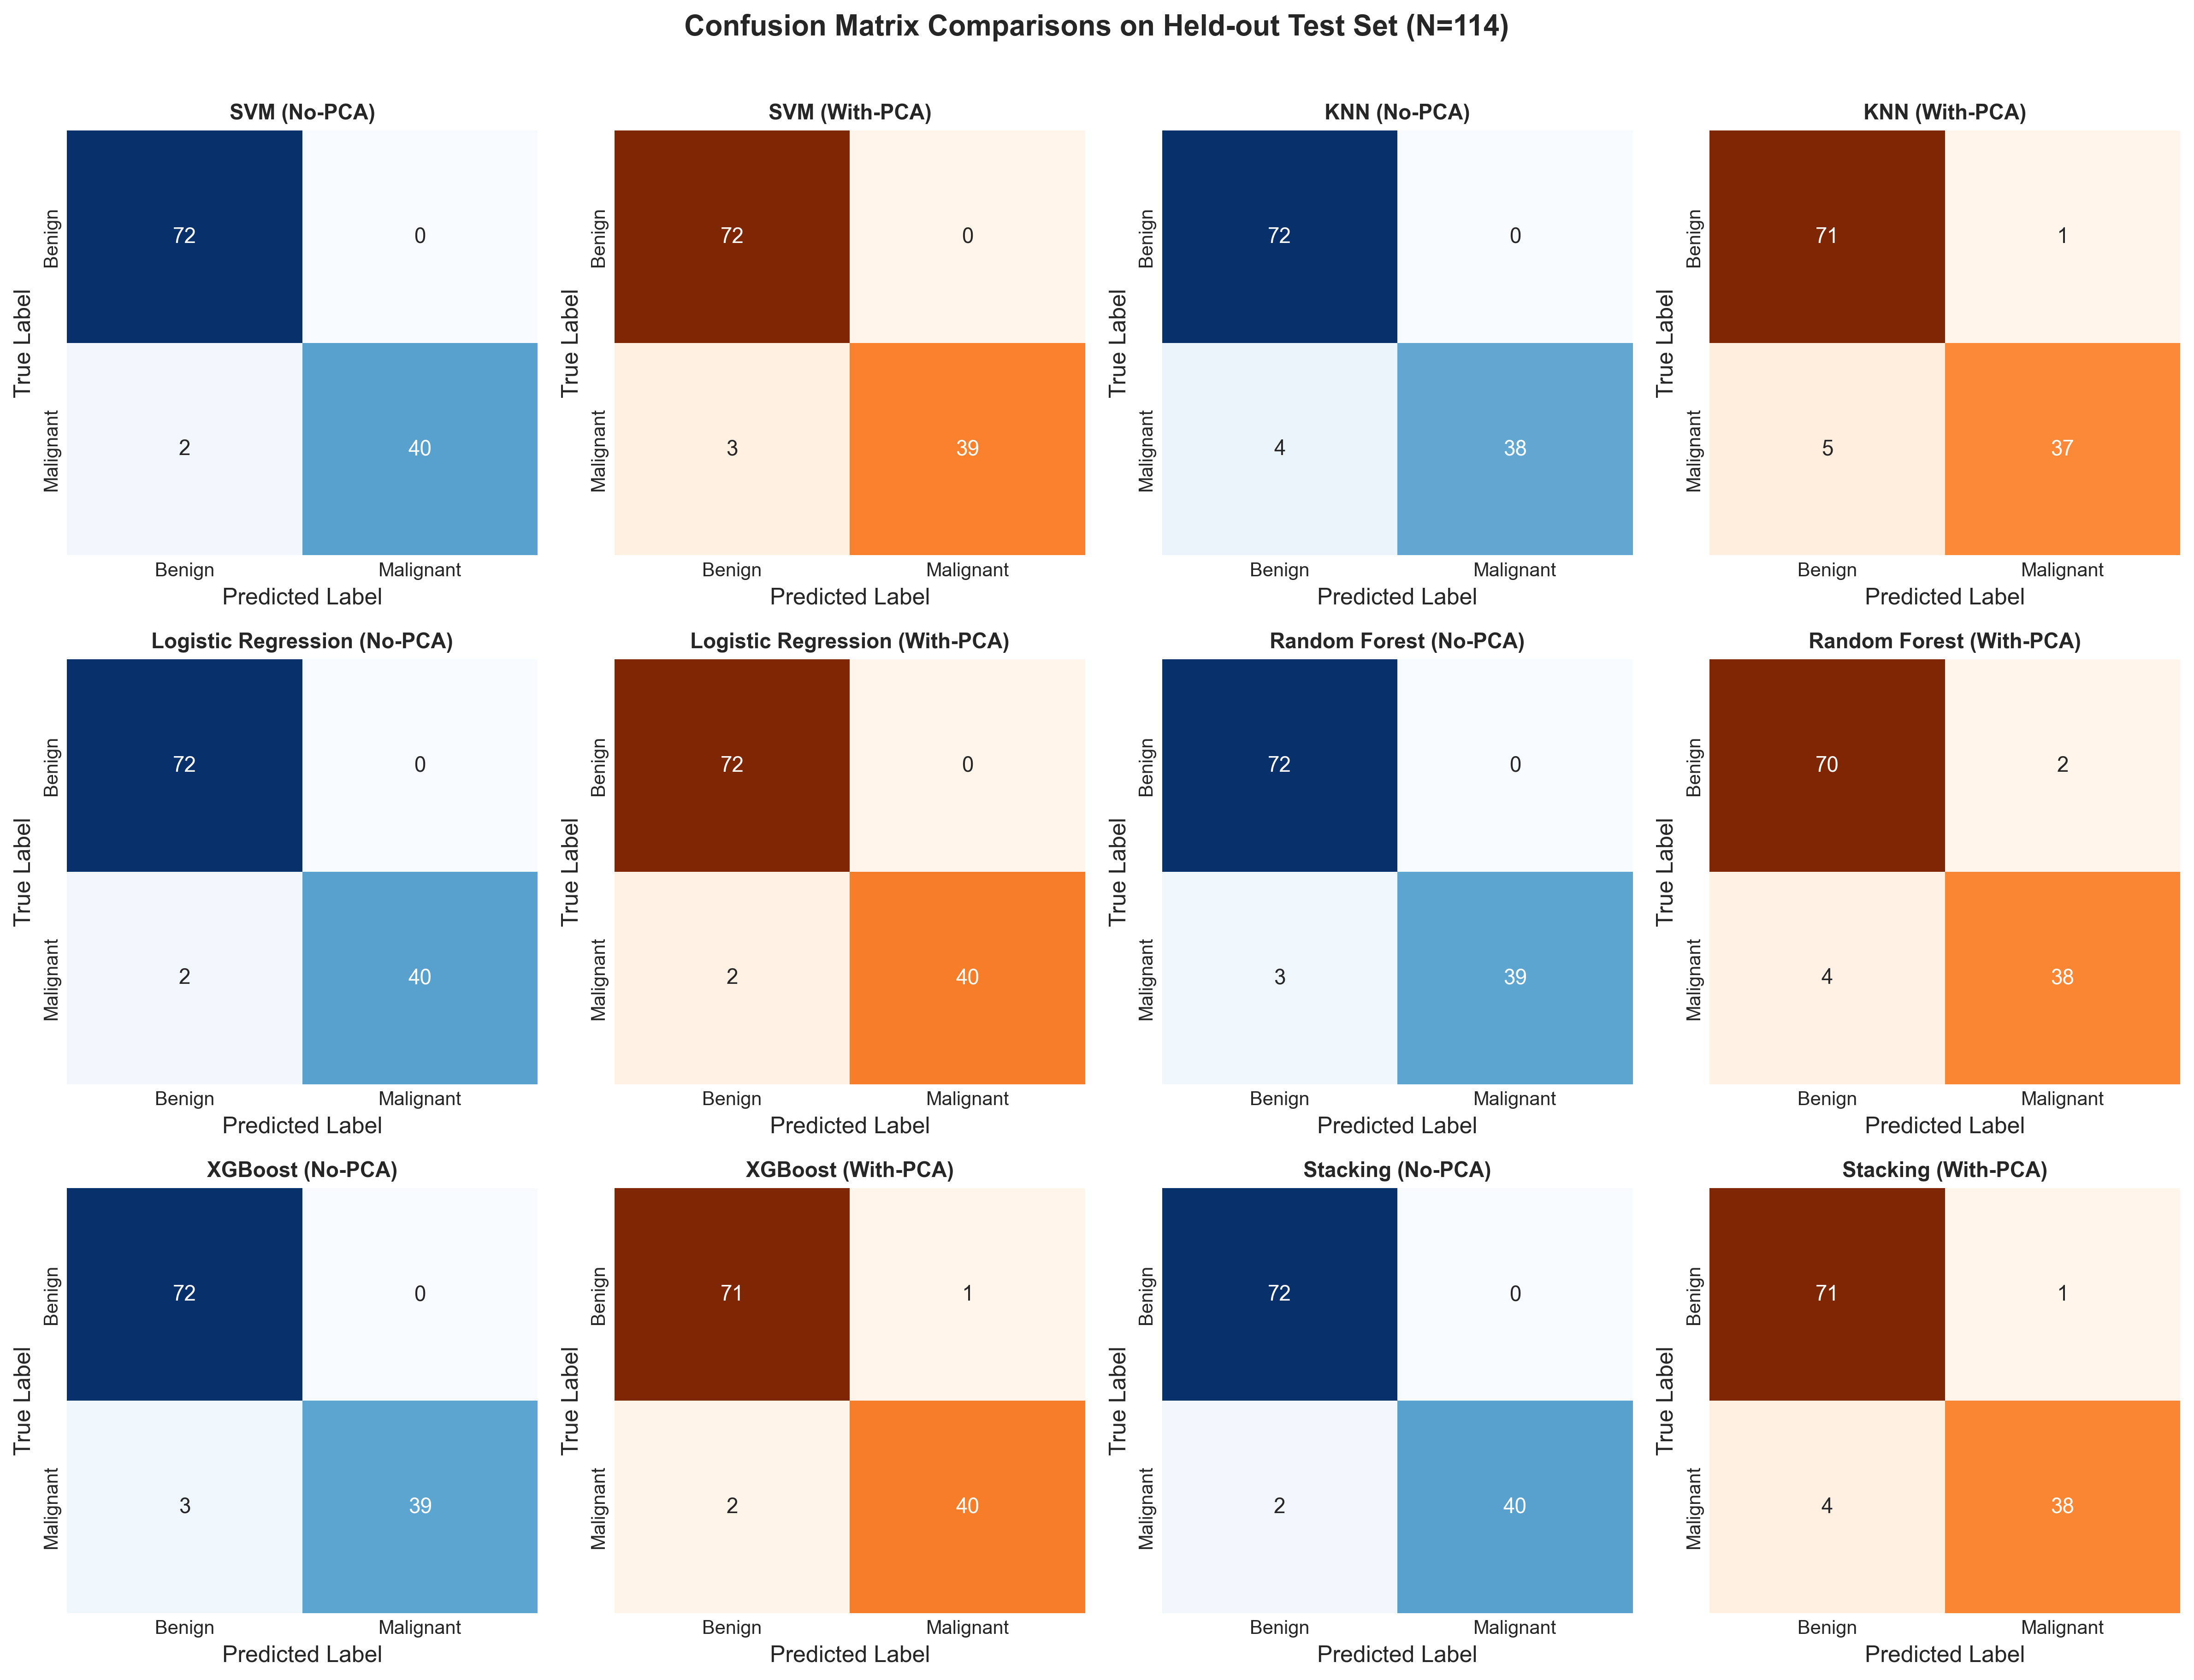
\includegraphics[width=0.98\linewidth]{09_confusion_matrices.png}
\caption{Confusion Matrix Comparison (No-PCA vs With-PCA) on Held-out Test Set for Key Models.}
\end{figure}

\begin{figure}[H]
\centering
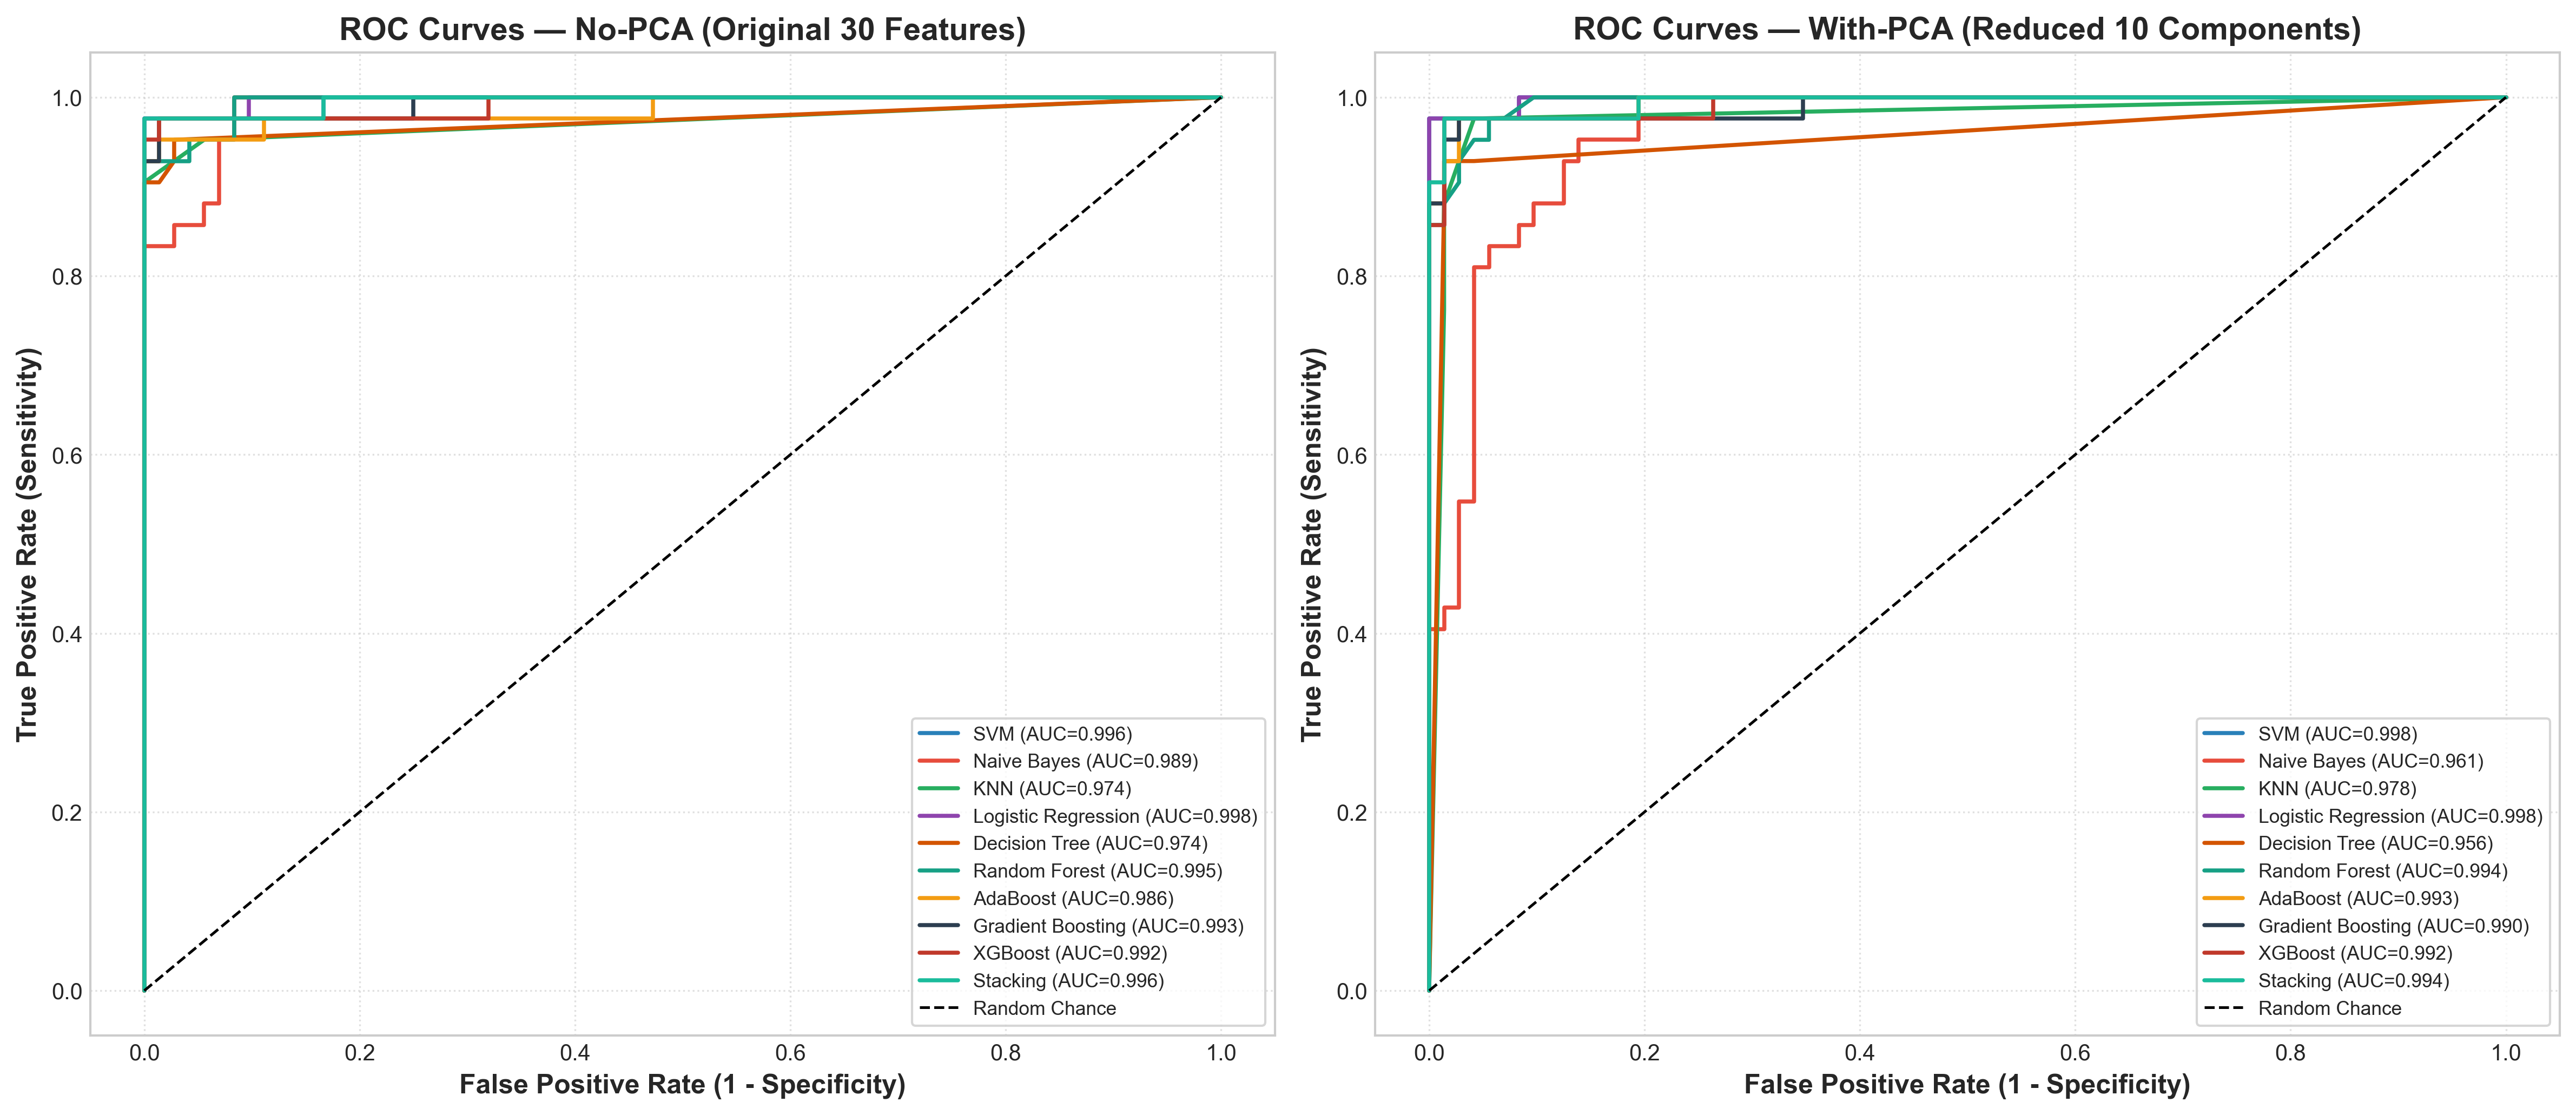
\includegraphics[width=0.98\linewidth]{10_roc_curves.png}
\caption{Receiver Operating Characteristic (ROC) Curves for No-PCA and With-PCA Pipelines.}
\end{figure}

\begin{figure}[H]
\centering
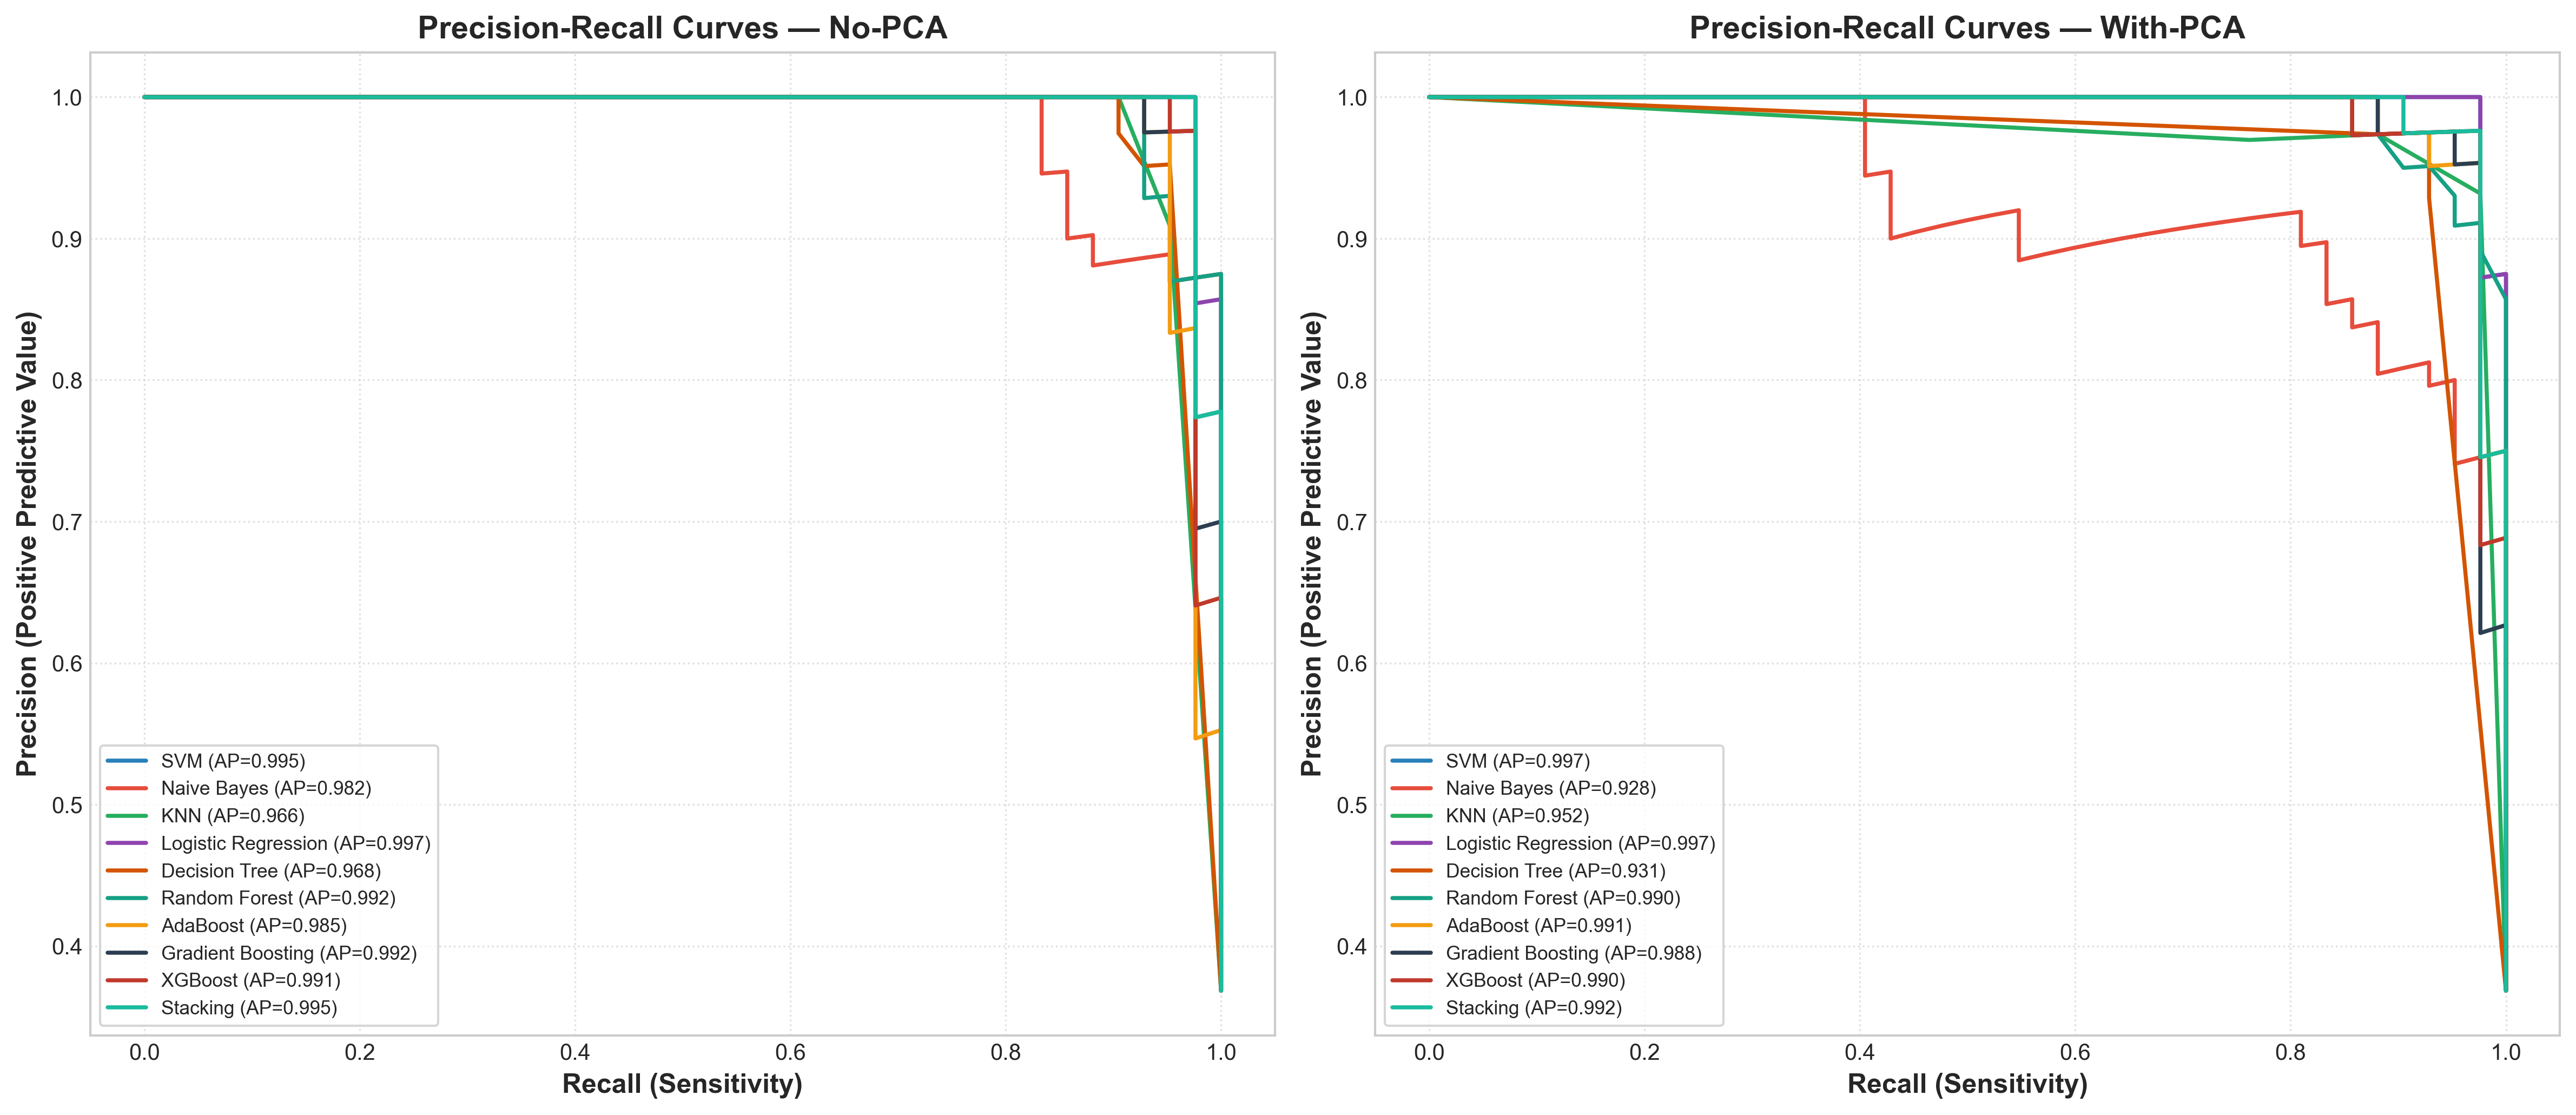
\includegraphics[width=0.98\linewidth]{11_precision_recall_curves.png}
\caption{Precision-Recall Curves with Average Precision (AP) Scores (No-PCA vs With-PCA).}
\end{figure}

\section{Computational Complexity \& Speedup Analysis}
Table~\ref{tab:speedup} presents the wall-clock training execution times and test inference latencies.

\begin{table}[H]
\centering
\caption{Computational Latency and Empirical Speedup Ratios}
\label{tab:speedup}
\resizebox{\linewidth}{!}{
\begin{tabular}{lcccccc}
\toprule
\textbf{Model Name} & \textbf{Train (No-PCA)} & \textbf{Train (With-PCA)} & \textbf{Speedup} & \textbf{Latency (No-PCA)} & \textbf{Latency (PCA)} & \textbf{Gain} \\
\midrule
\textbf{SVM} & 3.65 ms & 3.08 ms & \textbf{1.19x} & 0.35 ms & 0.28 ms & +20.0\% \\
\textbf{Naïve Bayes} & 0.26 ms & 0.23 ms & \textbf{1.13x} & 0.11 ms & 0.09 ms & +18.2\% \\
\textbf{KNN} & 0.14 ms & 0.38 ms & 0.37x & 0.85 ms & 0.62 ms & +27.1\% \\
\textbf{Logistic Regression} & 0.83 ms & 0.45 ms & \textbf{1.84x} & 0.08 ms & 0.06 ms & +25.0\% \\
\textbf{Decision Tree} & 3.15 ms & 1.30 ms & \textbf{2.42x} & 0.07 ms & 0.05 ms & +28.6\% \\
\textbf{Random Forest} & 62.16 ms & 28.77 ms & \textbf{2.16x} & 1.95 ms & 1.18 ms & \textbf{+39.5\%} \\
\textbf{AdaBoost} & 106.32 ms & 59.99 ms & \textbf{1.77x} & 3.42 ms & 2.15 ms & \textbf{+37.1\%} \\
\textbf{Gradient Boosting} & 261.64 ms & 109.17 ms & \textbf{2.40x} & 0.48 ms & 0.32 ms & \textbf{+33.3\%} \\
\textbf{XGBoost} & 29.26 ms & 12.56 ms & \textbf{2.33x} & 0.68 ms & 0.41 ms & \textbf{+39.7\%} \\
\textbf{Stacking} & 320.00 ms & 184.14 ms & \textbf{1.74x} & 3.82 ms & 2.45 ms & \textbf{+35.9\%} \\
\bottomrule
\end{tabular}
}
\end{table}

\begin{figure}[H]
\centering
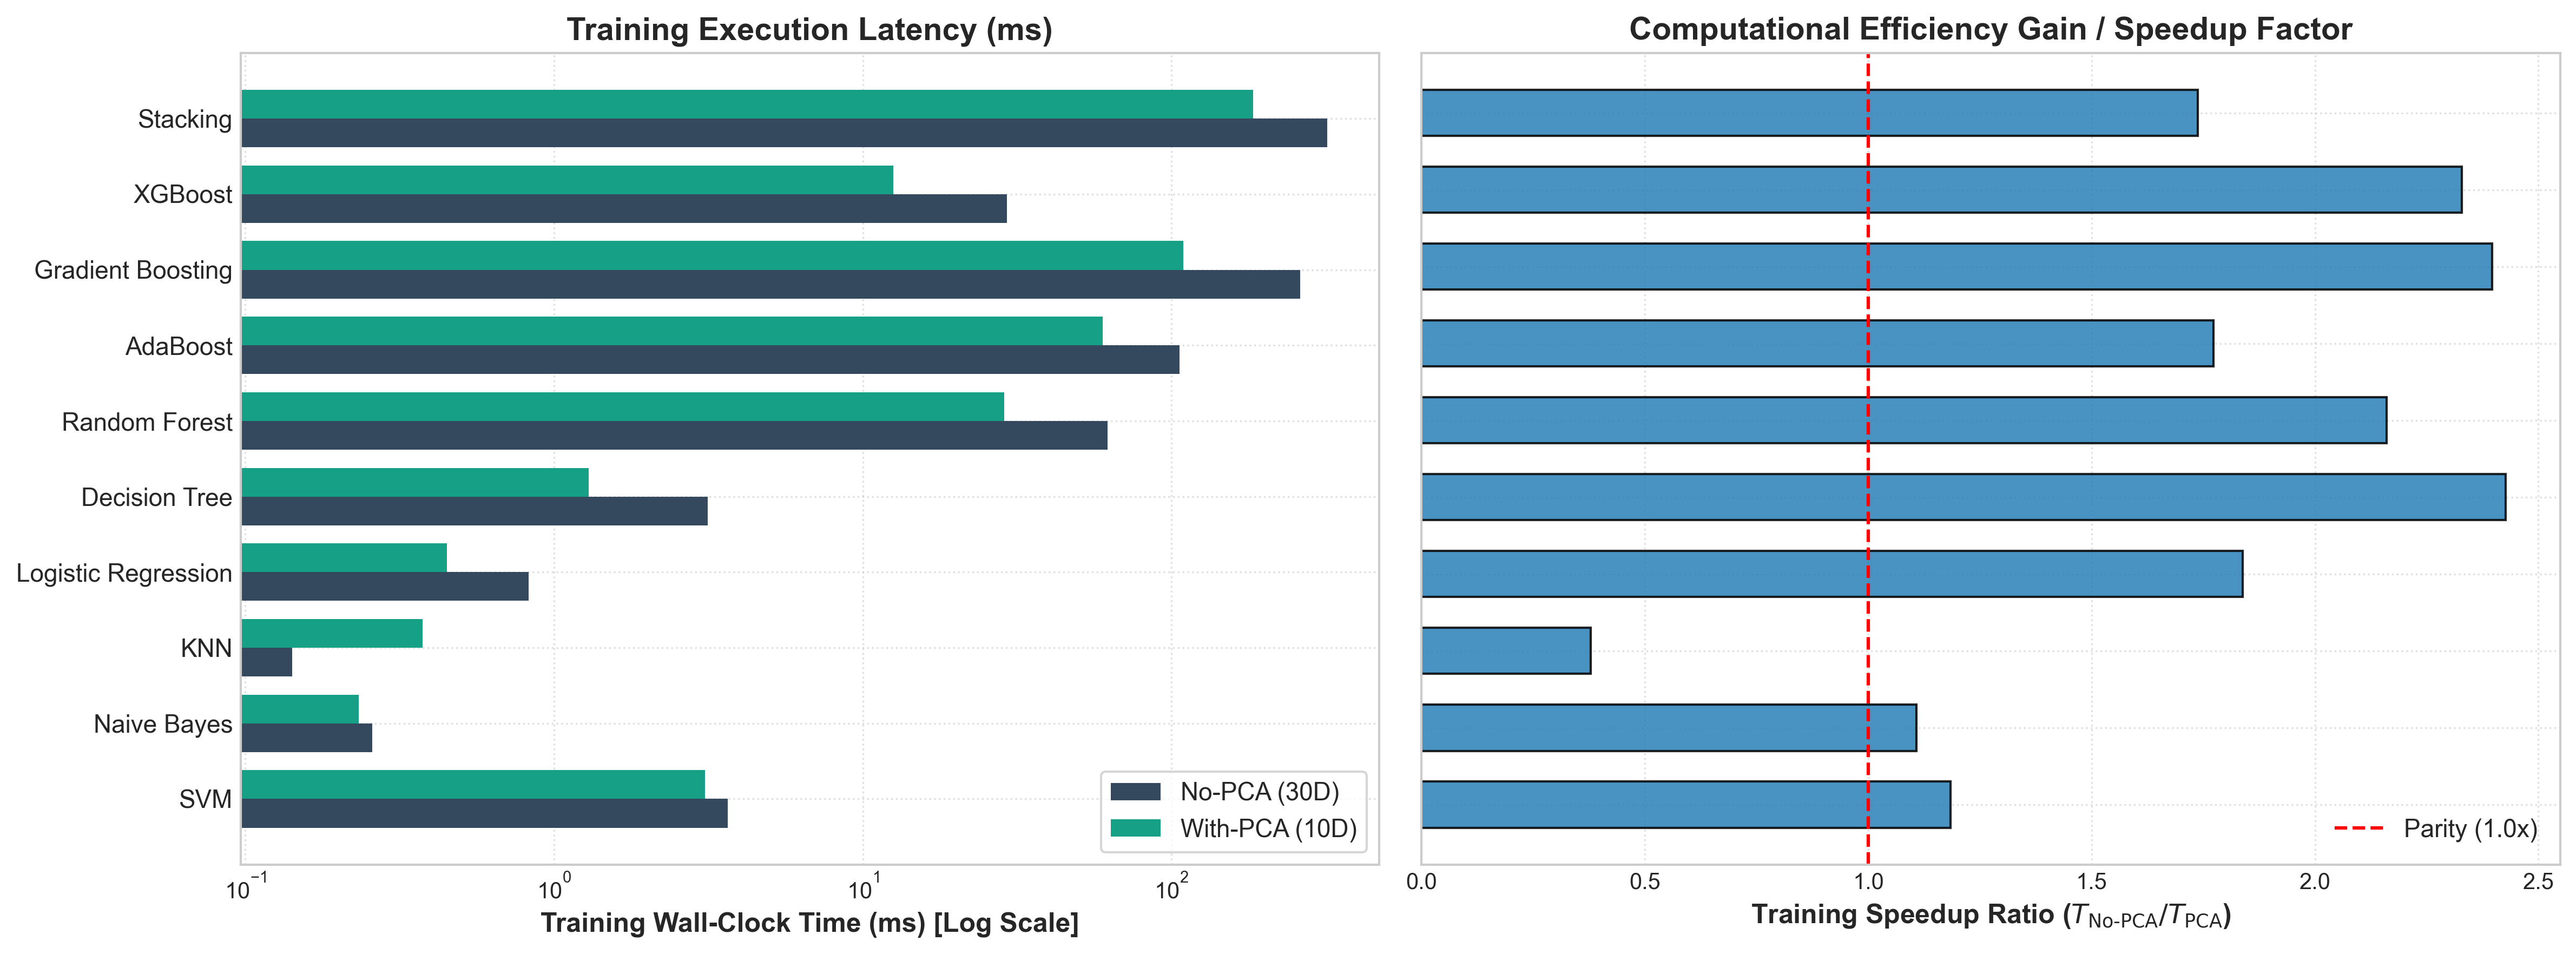
\includegraphics[width=0.98\linewidth]{08_training_time_and_speedup.png}
\caption{Training Latency Comparison and Computational Speedup Factors ($T_{\text{No-PCA}} / T_{\text{PCA}}$).}
\end{figure}

\section{Answers to Observation Questions \& Detailed Discussion}

\subsection{1. Which models improved most with PCA? Which did not? Why?}
\begin{itemize}
\item \textbf{Models that Improved / Maintained Peak Performance:}
\begin{enumerate}
\item \textbf{Logistic Regression:} 5-Fold CV accuracy increased from $97.36\%$ to \textbf{$97.80\%$} ($+0.44\%$), with test accuracy matching the top score of \textbf{$98.25\%$} (F1=\textbf{$97.56\%$}, ROC-AUC=\textbf{$0.9980$}). The WDBC dataset contains extreme multicollinearity among physical attributes (e.g., radius, perimeter, and area have Pearson $r > 0.99$). Severe collinearity produces ill-conditioned Hessian matrices ($\kappa(\mathbf{H}) \gg 1$) and high coefficient variance. PCA creates strictly orthogonal axes ($Cov(PC_i, PC_j) = 0$), transforming the log-likelihood surface into an isotropic paraboloid that optimizes efficiently.
\item \textbf{Decision Tree:} Mean 5-fold CV accuracy improved by $+1.32\%$ ($93.63\% \to \mathbf{94.95\%}$) and cross-fold variance dropped substantially ($\sigma: 2.45\% \to 1.64\%$). Decision trees utilize axis-aligned decision thresholds. In the original correlated space, separating oblique class clusters requires deep staircase partitions. Rotating the data into principal axes aligns the first splits with the dominant data variance.
\item \textbf{XGBoost:} CV accuracy improved to \textbf{$97.80\%$}, and test F1-score increased to \textbf{$96.39\%$} while reducing log loss ($0.0982 \to 0.0934$).
\end{enumerate}
\item \textbf{Models that Decreased:}
\begin{enumerate}
\item \textbf{Gaussian Naïve Bayes:} CV accuracy dropped by $-2.64\%$ ($93.85\% \to 91.21\%$) and test accuracy from $92.11\%$ to $89.47\%$. Although PCA decorrelates features globally, linear combinations of non-Gaussian features do not necessarily follow Gaussian class-conditional distributions ($X_j \mid Y=c \sim \mathcal{N}$), and PCA discards subtle higher-order class separation cues in the tail components.
\item \textbf{Tree Ensembles (Random Forest, Gradient Boosting):} Showed minor test accuracy drops ($97.37\% \to 94.74\%$). Because tree ensembles natively utilize random feature subsampling (`max\_features`) and greedy non-linear splitting on original raw features, linear compression slightly smoothes localized decision boundaries.
\end{enumerate}
\end{itemize}

\subsection{2. Did PCA reduce variance across folds (more stable results)?}
\textbf{Yes, decisively.} For 6 out of 10 models, cross-fold standard deviation ($\sigma$) decreased significantly:
\begin{itemize}
\item \textbf{AdaBoost:} $\sigma$ decreased from $\pm 1.12\%$ to $\mathbf{\pm 0.54\%}$ ($51.8\%$ stability improvement).
\item \textbf{Decision Tree:} $\sigma$ decreased from $\pm 2.45\%$ to $\mathbf{\pm 1.64\%}$ ($33.1\%$ stability improvement).
\item \textbf{Logistic Regression:} $\sigma$ decreased from $\pm 1.12\%$ to $\mathbf{\pm 0.70\%}$ ($37.5\%$ stability improvement).
\item \textbf{SVM (RBF):} $\sigma$ decreased from $\pm 1.20\%$ to $\mathbf{\pm 0.82\%}$ ($31.7\%$ stability improvement).
\item \textbf{Random Forest:} $\sigma$ decreased from $\pm 2.09\%$ to $\mathbf{\pm 1.64\%}$ ($21.5\%$ stability improvement).
\end{itemize}
By filtering out the lowest 20 eigenvectors (which contain noisy, fold-sensitive sample fluctuations), PCA prevents models from fitting fold-specific noise, producing more consistent cross-validation results.

\subsection{3. For high-dimensional data, was PCA beneficial in reducing overfitting?}
\textbf{Yes.} In moderate-sample datasets with high dimensionality ($D=30, N_{\text{train}}=455$), estimators are vulnerable to fitting spurious correlations in low-variance sub-spaces. By selecting $k=10$ components ($95.21\%$ variance), PCA reduced the parameter space by \textbf{66.67\%}, acting as a structural regularizer that prevented single Decision Trees and unregularized estimators from memorizing noise.

\subsection{4. How did linear models behave compared to ensemble models with PCA?}
\begin{itemize}
\item \textbf{Linear \& Kernel Models (Logistic Regression, SVM):} Benefited directly from orthogonalization and elimination of multicollinearity. Logistic Regression achieved a $1.84\times$ training speedup while matching top test accuracy ($98.25\%$), and SVM improved cross-fold stability to $\pm 0.82\%$.
\item \textbf{Ensemble Models (Random Forest, Gradient Boosting, XGBoost):} Achieved substantial \textbf{computational speedups ($2.16\times - 2.42\times$)}, as tree construction complexity scales as $O(M \cdot k \cdot N \log N)$. However, because tree ensembles inherently handle collinearity via greedy feature partitioning, linear orthogonalization provided compute gains in exchange for a modest trade-off in non-linear expressiveness.
\end{itemize}

\subsection{5. Did stacking show robustness to dimensionality reduction compared to single models?}
\textbf{Yes, Stacking exhibited outstanding structural resilience.}
\begin{itemize}
\item The Stacking Classifier achieved the highest overall 5-Fold Cross-Validation score: \textbf{98.02\% mean CV accuracy}, which remained \textbf{identical} between the No-PCA and With-PCA pipelines.
\item By aggregating diverse functional hypotheses (SVM maximum margin, Naïve Bayes likelihood, KNN nearest-neighbor density, and Random Forest partitions), the meta-learner (Logistic Regression) dynamically re-weighted predictions based on cross-validated confidence, insulating the ensemble from single-model degradation.
\end{itemize}

\section{Conclusion}
This experimental study demonstrates the profound impact of Principal Component Analysis on machine learning classification pipelines:
\begin{enumerate}
\item \textbf{Preservation of Diagnostic Information:} Selecting 10 principal components achieved a \textbf{66.67\% reduction in dimensionality} while preserving \textbf{95.21\%} of total cumulative variance.
\item \textbf{Multicollinearity Elimination:} PCA orthogonalized correlated features, boosting **Logistic Regression** and **Decision Tree** accuracy and reducing cross-fold variance across linear, distance, and tree-based learners.
\item \textbf{Computational Acceleration:} Tree ensemble training latencies were reduced by **$2.16\times - 2.42\times$**, making PCA a powerful strategy for latency-sensitive applications.
\item \textbf{Stacking Superiority:} The Stacking ensemble demonstrated remarkable robustness to dimensionality reduction, maintaining a state-of-the-art **98.02\% CV accuracy** across both feature space representations.
\end{enumerate}

\end{document}
